\documentclass[11pt]{article}

% --- Core Academic Packages ---
\usepackage[utf8]{inputenc}
\usepackage{amsmath, amsthm, amssymb, amsfonts} % Essential for formal econometric math
\usepackage{booktabs}                           % Publication-quality tables (\toprule, \midrule, \bottomrule)
\usepackage{threeparttable}                    % Crucial for robust standard error notes below tables
\usepackage{graphicx}                          % For visual proofs/plots
\usepackage{subcaption}                        % Panel A / Panel B structural layouts
\usepackage{geometry}                           % Standard margins
\usepackage{setspace}                           % Double/1.5 spacing for referee drafts
\usepackage[toc,page]{appendix}                % Formal appendix formatting
\usepackage[colorlinks=true, linkcolor=blue, citecolor=blue]{hyperref}
\usepackage[backend=biber, style=authoryear, maxcitenames=2, uniquename=false]{biblatex}
\usepackage{enumitem}

\geometry{a4paper, margin=0.70in}

\addbibresource{bib.bib}

\title{\textbf{Economic Development, a Political Materialism perspective}}
\author{\textbf{Carlos Gustavo Salas Flores} \\ \small Beijing Normal University}
\date{Oct 2026}

\begin{document}

\maketitle

% =========================================================================
% 1. BACKGROUND
% =========================================================================
\section{Background}
\label{sec:background}

\subsection{The measurement problem in comparative political economy}

Recent economic models use indicators such as V-Dem and Polity-V to capture latent political variables. \textcite{treier_jackman_2008} identified substantial measurement error in Polity-V's democracy scores and showed how that error can distort inference. \textcite{little_meng_2024} likewise found that recent claims of democratic backsliding receive little support from objective records of election results, electoral competitiveness, and journalists jailed or killed. Their results point to changes in expert assessments even when the underlying measures remain stable.

The problem extends beyond research on democracy. A theory of economic development built on indicators partly shaped by expert judgment also inherits their measurement error. That concern motivates the approach taken here.

\subsection{The institutional theory of development and its limits}

Acemoglu, Johnson, and Robinson (hereafter AJR) developed an influential theory of Inclusive and Extractive Institutions to explain why territories with similar material conditions can follow very different development paths, as in Nogales, Arizona, and Nogales, Sonora \parencite{acemoglu_johnson_robinson_2001,acemoglu_johnson_robinson_2005,acemoglu_robinson_2012}. Their account offers a thin theory of the state: economic indicators and expert opinions supply the basis for classifying a nation as Inclusive (II) or Extractive (EI). Two difficulties follow. \textit{I) Circular measurement.} Inclusive Institutions are defined by outcomes such as low expropriation rates and secure property rights, which the classification is then used to explain. If Inclusive Institutions imply low expropriation ($A \to X$), observing low expropriation cannot establish the presence of Inclusive Institutions ($X \to A$). Because the outcome helped construct the classification, the classification cannot provide an independent explanation. \textit{II) Vague horizon.} AJR respond that Extractive Institutions may sustain inclusive economic policies for a time, although such economies are destined to fail eventually. With no time bound, continued success can always be described as ``not yet long term,'' leaving the claim unfalsifiable.

A related literature links democratization directly to growth. \textcite{acemoglu_naidu_restrepo_robinson_2019} find that democratic transitions raise subsequent growth. Their measures of democracy remain vulnerable to the concerns raised by \textcite{little_meng_2024}: an estimated relationship may reflect changes in expert assessments as well as changes in the economies being assessed. A direct account of state structures and international positions would avoid that dependence on contested expert-coded indices.

\subsection{Research question and hypotheses}

This work asks: \emph{which changes in a country's political and international situation produce major economic discontinuities---sharp breaks in a country's economic trajectory, whether downward or upward?} Answering this question requires distinctions among events commonly grouped under ``regime change'': replacement of officeholders, replacement of the coalition sustaining them, changes in formal rules of access to power, transformations of the effective structure of political power, restructuring of the state apparatus, policy change, and shifts in external alignment. Section~\ref{sec:framework} defines each term.

These concepts yield three testable hypotheses.

\begin{itemize}
    \item $H_1$ on government turnover: For any two countries $A$ and $B$ with comparable material endowments and similar external alignment, government turnover---and even nominal regime change---that leaves the effective structure of political power untouched will not produce a major economic discontinuity.
    \item $H_2$ on external realignment: For any two such countries, variation in major economic discontinuities tracks variation in external alignment rather than variation in domestic political events. The sign of the discontinuity depends on the type of realignment: severance from a dominant power's sphere of influence deprives the state of material capabilities and produces \emph{disruption}, whereas entry into a richer sphere supplies material capabilities and produces \emph{acceleration}.
    \item $H_3$ on the interaction of domestic and international change: A country that undergoes domestic political change will experience a major economic discontinuity only when that change coincides with an external realignment; and external realignment produces a major discontinuity---disruption or acceleration, according to its type---whether or not domestic political change accompanies it.
\end{itemize}

$H_3$ is logically independent of $H_1$ and $H_2$ and makes a stronger claim, so it requires a separate test. Section~\ref{sec:hypotheses} derives the observable implications of all three hypotheses in a comparative design.

% =========================================================================
% 2. THEORETICAL FRAMEWORK
% =========================================================================
\section{Theoretical Framework}
\label{sec:framework}

Five questions organize the framework: \textbf{who governs}, \textbf{how political power is organized}, \textbf{through which permanent institutions power is exercised}, \textbf{where the state sits internationally}, and \textbf{what outcomes follow}.

\subsection{Units of analysis}

\begin{itemize}
	\item A \emph{country} is a territorial, geographical, demographic, or economic unit. The term applies to comparisons of geographical conditions or economic performance; analysis of the state as a political organization requires a different unit \parencite{linz_stepan_1996,waltz_1979}.
	\item The \emph{state} has two related senses here. Domestically, it is the durable political organization possessing administrative and coercive authority over a territory \parencite{weber1922wirtschaft,hobbes1651leviathan}. Internationally, it is the corporate actor whose alignment and position change relative to other states \parencite{waltz_1979,mearsheimer_2001}. Publicly funded bodies taken collectively, like the incumbent government, fall outside this definition.
	\item The \emph{international system} is the wider structure within which states operate. Its anarchy and distribution of capabilities, especially among great powers, constrain behavior without acting on their own \parencite{waltz_1979,mearsheimer_2001}. For cases situated within a particular regional distribution of power, the relevant unit is the \emph{regional subsystem} \parencite{buzan_waever_2003}.
\end{itemize}

\subsection{Domestic political elements and actors}

\begin{itemize}
	\item The \emph{government} (or incumbent administration) denotes the persons and organizations currently holding governing office: presidents, prime ministers, ministers, and, where relevant, the ruling coalition. It answers ``who governs?''. Policies and international behavior belong to the government's actions; the definition itself concerns occupancy of office \parencite{linz_stepan_1996}.
	\item The \emph{ruling coalition} is the wider set of parties, elites, and organized groups that sustain the government in power. A change of president or governing party can leave this coalition intact \parencite{bueno_de_mesquita_2003}.
	\item The \emph{political regime} comprises the rules and institutional arrangements governing access to political power, the distribution of authority among institutions, competition for office, and control or accountability over rulers; it answers ``how is political power formally organized?'' \parencite{linz_stepan_1996,linz_2000}.
	\item The \emph{structure of political power}, by contrast, captures the \emph{effective} organization and control of power: the actual separation or concentration of powers, the independence of representation, the party--state relationship, and the capacity of citizens or rival elites to control rulers \parencite{garciatrevijano2010}. Formal regime change can coexist with continuity in this structure. Garc{\'i}a-Trevijano's party-state (\emph{Estado de partidos}) illustrates the distinction: state-integrated parties collectively control political power behind formally democratic institutions \parencite{garciatrevijano2010}.
	\item \emph{Political parties} may participate in government, opposition, or the ruling coalition. A party's participation in opposition or in the ruling coalition does not by itself make it part of the government \parencite{sartori_1976}.
	\item The \emph{state apparatus} is the durable administrative, coercive, judicial, and fiscal machinery through which political authority is exercised \parencite{weber1922wirtschaft,althusser_1971}. It has three main components:
	\begin{itemize}
		\item the \emph{coercive apparatus} (armed forces, police, security services; \textcite{tilly_1990,althusser_1971}),
		\item the \emph{administrative apparatus} (ministries and public bureaucracy; \textcite{weber1922wirtschaft}), and
		\item the \emph{judicial apparatus} (courts and related institutions; \textcite{weber1922wirtschaft,garciatrevijano2010}).
	\end{itemize}
	\item The \emph{public sector} is a residual category for publicly owned or funded bodies such as hospitals, schools, and state companies. Inclusion in this category alone establishes neither membership in the core state apparatus nor strategic political agency.
\end{itemize}

\subsection{International actors and structural elements}

\begin{itemize}
	\item A \emph{great power} is a state with military capabilities large enough to play a major role in the distribution of power \parencite{mearsheimer_2001}.
	\item In asymmetric relationships, the \emph{dominant power} is the stronger state and the \emph{subordinate state} the one whose security, alignment, or foreign-policy choices are substantially constrained by it. Such international relationships are hierarchical even when the states remain formal equals \parencite{lake_2009}.
	\item A \emph{hegemon} is a state powerful enough to dominate the others in the relevant system or region \parencite{mearsheimer_2001}. An \emph{aligned state} coordinates its external orientation with another power; subordination requires more than alignment \parencite{walt_1987}.
	\item A \emph{sphere of influence} is a determinate region or relationship in which an external power exercises predominant influence and limits the independence of the political entities within it. Predominant influence can exist without complete control \parencite{keal_1983,hast_2014}.
	\item A state's \emph{external alignment} is its position vis-\`a-vis great powers, alliances, and spheres of influence \parencite{walt_1987}. Its \emph{position within the international structure} is its location relative to other powers. Realignment changes that position; structural change requires a change in the distribution of capabilities \parencite{waltz_1979}.
\end{itemize}



\subsection{An event taxonomy}

The literature often uses ``regime change'' for several different events at once. This framework separates them into the following categories.

\begin{itemize}
	\item \emph{Government turnover} replaces the persons or parties holding office \parencite{bueno_de_mesquita_2003}.
	\item \emph{Ruling-coalition change} replaces the wider set of actors whose support sustains rule \parencite{bueno_de_mesquita_2003}.
	\item \emph{Regime change} alters the formal rules governing access to and organization of political power \parencite{linz_stepan_1996}. 
	\item A \emph{transformation of the power structure} alters the effective concentration, separation, representation, or control of political power. This category separates nominal regime change from deeper structural continuity \parencite{garciatrevijano2010}.
	\item \emph{State-apparatus restructuring} transforms the durable administrative, coercive, judicial, or fiscal machinery of the state \parencite{skocpol_1979,althusser_1971}. 
	\item \emph{Policy change} alters what the government does---its settings, instruments, or overarching goals---and belongs to a separate category from both turnover and regime change \parencite{hall_1993}.
	\item An \emph{external realignment} changes a state's alliance, dominant-power relationship, or sphere of influence \parencite{walt_1987}. A \emph{systemic power shift}, in contrast, changes the overall distribution of capabilities among states \parencite{gilpin_1981,waltz_1979}.
\end{itemize}

These distinctions allow for two possibilities that aggregate accounts often obscure. Turnover or nominal regime change can leave the underlying structure of political power intact, and external realignment can occur with or without a systemic power shift.

\subsection{Outcomes and conditioning conditions}

The dependent phenomenon is a \emph{major economic discontinuity}: a sharp and sustained break in a country's prior economic trajectory, in either direction. Its negative form, \emph{economic disruption}, covers output collapse, inflation, or capital flight \parencite{rodrik_1999}; its positive form, \emph{economic acceleration}, covers sustained take-off and convergence with richer economies. The sign of the discontinuity follows the direction of the change in material capabilities. Severance withdraws the benefits of a dominant-power relationship, such as market access, capital, and security guarantees; entry supplies them \parencite{lake_2009,gilpin_1981}. \emph{Material endowments} (geography, natural resources, environment, population) are relatively durable conditions that constrain economic and strategic possibilities \parencite{diamond_1997}. \emph{Material capabilities} are the resources a state can mobilize, making them politically usable capacities \parencite{mearsheimer_2001}.

The framework links two levels of analysis. Domestically, incumbent governments govern with the support of ruling coalitions, within a political regime and an effective structure of political power, and through a durable state apparatus. Internationally, states hold an external alignment and occupy a position within the international structure, especially in relation to great powers and their spheres of influence. Material endowments and capabilities condition their economic and military outcomes.

% =========================================================================
% 3. LITERATURE REVIEW
% =========================================================================
\section{Literature Review}
\label{sec:lit_review}

Four bodies of literature bear on the research question.

\paragraph{Institutions and development.} AJR's institutional theory \parencite{acemoglu_johnson_robinson_2001,acemoglu_johnson_robinson_2005,acemoglu_robinson_2012} and the democratization--growth literature \parencite{acemoglu_naidu_restrepo_robinson_2019} locate the sources of development in domestic institutions. Their institutional measures depend on expert-coded indices of contested reliability \parencite{treier_jackman_2008,little_meng_2024} and, in the case discussed in Section~\ref{sec:background}, on classifications vulnerable to circularity and unfalsifiability. Both strands also conflate the replacement of rulers with transformation of the power structure, which can lead them to attribute too much to visible domestic political change.

\paragraph{Regimes, power structures, and the state.} Comparative politics provides finer domestic distinctions. \textcite{linz_stepan_1996} and \textcite{linz_2000} separate state, regime, and government; \textcite{garciatrevijano2010} adds the effective structure of political power and the party-state paradigm; \textcite{sartori_1976} and \textcite{bueno_de_mesquita_2003} clarify parties and support coalitions; and \textcite{weber1922wirtschaft}, \textcite{althusser_1971}, \textcite{tilly_1990}, and \textcite{skocpol_1979} theorize the durable state apparatus that persists through changes of rulers. \textcite{hall_1993} further distinguishes orders of policy change, reminding us that an observable policy shift need not signal deep political change.

\paragraph{International structure and hierarchy.} Structural realism treats states as like units positioned within an anarchic system whose distribution of capabilities constrains them \parencite{waltz_1979}, with great powers competing for power and regional hegemony \parencite{mearsheimer_2001}. Work on alignment and alliance choices \parencite{walt_1987}, hierarchy between dominant and subordinate states \parencite{lake_2009}, spheres of influence \parencite{keal_1983,hast_2014}, regional security complexes \parencite{buzan_waever_2003}, and systemic power shifts \parencite{gilpin_1981} supplies the international side of the framework.

\paragraph{Material conditions and shocks.} Geographical and environmental endowments condition development possibilities \parencite{diamond_1997}, and population and wealth convert into latent and military power \parencite{mearsheimer_2001}. \textcite{rodrik_1999} shows that domestic conflict-management institutions mediate growth collapses after external shocks. For the present argument, this finding directs attention to the interaction between external position and domestic political organization; regime labels alone offer little explanatory leverage.

The thesis joins these literatures through two distinctions: domestic events that change rulers are separated from those that change power structures, and a state's positional realignment is separated from systemic power shifts. Existing accounts have not combined these distinctions to explain major economic discontinuities. The hypotheses stated in Section~\ref{sec:background} develop the resulting claim.

% =========================================================================
% 4. HYPOTHESES AND EMPIRICAL IMPLICATIONS
% =========================================================================
\section{Hypotheses and Empirical Implications}
\label{sec:hypotheses}

The three hypotheses translate into the comparative design of Table~\ref{tab:design}. Cases are selected as pairs of countries with comparable material endowments; the design then crosses (rows) the type of domestic political change with (columns) the type of external realignment: none, severance from a dominant power's sphere, or entry into a richer sphere.

\begin{table}[htbp]
\centering
\begin{threeparttable}
\caption{Predicted economic discontinuities by type of political and international change}
\label{tab:design}
\begin{tabular}{@{}p{0.26\linewidth}p{0.20\linewidth}p{0.22\linewidth}p{0.22\linewidth}@{}}
\toprule
 & No external realignment & Severance from a sphere & Entry into a richer sphere \\
\midrule
Government turnover / nominal regime change only & No major discontinuity ($H_1$) & Disruption ($H_2$, $H_3$) & Acceleration ($H_2$, $H_3$) \\
Power-structure transformation or apparatus restructuring & Ambiguous; out of scope of $H_1$ & Disruption ($H_2$) & Acceleration ($H_2$) \\
No domestic political change & No major discontinuity & Disruption ($H_2$, $H_3$) & Acceleration ($H_2$, $H_3$) \\
\bottomrule
\end{tabular}
\begin{tablenotes}
\small
\item Note: Predictions assume comparable material endowments across compared cases. \emph{Severance} means the loss of a dominant-power relationship's material benefits (market access, capital, security guarantees); \emph{entry} means gaining them \parencite{walt_1987,keal_1983,lake_2009}. Domestic event categories follow Section~\ref{sec:framework}.
\end{tablenotes}
\end{threeparttable}
\end{table}

The design is falsifiable for three reasons. Event categories are defined independently of outcomes, allowing cases to be classified without circularity. $H_1$ fails if matched cases show a major discontinuity after turnover that left the power structure and external alignment untouched. $H_2$ and $H_3$ fail if major discontinuities appear without realignment, if realignment leaves the economic trajectory intact, or if the outcome has the wrong sign---acceleration after severance or disruption after entry into a richer sphere. Nor can $H_3$ be reduced to the biconditional claim that discontinuity occurs if and only if domestic change coincides with external realignment; $H_1$ and $H_2$ do not entail that stronger proposition. $H_3$ thus stands as a separate prediction for matched-country tests. Two coding rules apply throughout: an attributed outcome must postdate the realignment, and the acceleration threshold must be symmetric to the disruption threshold.

% =========================================================================
% 5. METHODOLOGY
% =========================================================================
\section{Methodology}
\label{sec:methodology}

The empirical strategy combines comparative case analysis, which carries the causal narrative, with statistical analysis of the same predictions across a larger set of observations. Both use the same coding rules, and a failure in either layer counts against the theory.

\subsection{Comparative case analysis}

Matched pairs of countries with comparable material endowments provide the cases (Section~\ref{sec:hypotheses}). Coding follows the event taxonomy and outcome definitions in Section~\ref{sec:framework}, with a \emph{disruption} threshold adapted from \textcite{rodrik_1999} and a symmetric \emph{acceleration} threshold adapted from \textcite{hausmann_pritchett_rodrik_2005}. Both thresholds are fixed before case coding. Process tracing establishes the sequence of events within each case. Under the timing rule in Section~\ref{sec:hypotheses}, an outcome can be attributed to a realignment only when it occurs afterward. Table~\ref{tab:design} specifies the comparative design and its falsification criteria.

\subsection{Statistical analysis}

The statistical layer begins with a model-free description. Country-years are classified into the cells of Table~\ref{tab:design}; for each cell, we report the frequency of major economic discontinuities and mean growth after each type of realignment. The theory predicts concentration in the severance and entry columns with opposite signs, alongside a quiet no-realignment column regardless of domestic political events.

The second step is a linear regression on a country-year panel. Following \textcite{acemoglu_naidu_restrepo_robinson_2019}, the specification retains country and year fixed effects together with lags of the political variable. Observable event variables replace the expert-coded democracy index:
\begin{equation}
\begin{split}
g_{it} = \alpha_i + \lambda_t &+ \beta_1 \mathrm{Severance}_{it} + \beta_2 \mathrm{Entry}_{it} + \beta_3 \mathrm{Turnover}_{it} \\
&+ \beta_4 \mathrm{RegimeChange}_{it} + \beta_5 \mathrm{PowerStructure}_{it} + \gamma' X_{it} + \varepsilon_{it},
\end{split}
\label{eq:main}
\end{equation}
where $g_{it}$ is real GDP per capita growth in country $i$ in year $t$; $\alpha_i$ and $\lambda_t$ are country and year fixed effects; the event indicators equal one in the year of the event and are also included with lags, so that effects can materialize over several years \parencite{acemoglu_naidu_restrepo_robinson_2019}; and $X_{it}$ collects controls for the material channel (oil rents as a share of GDP, population, investment share). Standard errors are clustered by country.

The hypotheses translate into restrictions on the coefficients. $H_1$ predicts $\beta_3 = \beta_4 = 0$: turnover and nominal regime change alone have no effect. $H_2$ predicts $\beta_1 < 0$ (severance produces disruption) and $\beta_2 > 0$ (entry into a richer sphere produces acceleration). $H_3$ is examined by interacting the domestic event indicators with the realignment indicators. The coefficient on power-structure transformation, $\beta_5$, is left free, since the theory makes no claim about that row of Table~\ref{tab:design}.

The sample is restricted to the regions covered by the case survey---Latin America, the post-Soviet space, East Asia, and Europe---over 1960--2019; extending the panel to a global sample is left for later work. Robustness checks include alternative outcome thresholds, the exclusion of the systemic-shock years 1989--1991, and synthetic-control estimates for the two most extreme cases, Venezuela and Cuba \parencite{abadie_diamond_hainmueller_2010}.

\subsection{Coding rules}
\label{sec:coding}

All variables are coded from observable events using rules fixed in advance. The replication materials document the full protocol, whose three parts are summarized here.

\paragraph{Outcome thresholds.} A \emph{disruption} is coded when real GDP per capita contracts by at least 15 percent peak-to-trough within five years, or growth falls at least three percentage points below its prior five-year average for at least three years, or annual inflation exceeds 500 percent \parencite{rodrik_1999}. An \emph{acceleration} is coded when growth of at least 3.5 percent per year is sustained for at least eight years, at least two percentage points above the prior growth regime \parencite{hausmann_pritchett_rodrik_2005}. The thresholds are symmetric by construction and are fixed before any case is coded.

\paragraph{Domestic political events.} Turnover is coded from leader records \parencite{goemans_gleditsch_chiozza_2009}; regime change from constitutional events \parencite{elkins_ginsburg_melton_2009}. A \emph{transformation of the power structure}---the category that separates nominal regime change from deep structural change---is coded only when at least two of four dimensions change within a three-year window, each anchored to a primary legal or institutional act: the separation or concentration of powers in practice, the independence of representation, the fusion of ruling party and state, and the capacity to control rulers \parencite{garciatrevijano2010}.

\paragraph{External realignment.} Following \textcite{keal_1983}, a sphere of influence requires predominant influence; formal control is unnecessary. Membership requires documented influence in at least two of four indicator families: security ties \parencite{leeds_etal_2002,gibler_sarkees_2004}, economic dependence \parencite{imf_dots}, institutional bloc membership, and coercion \parencite{felbermayr_etal_2020}. \emph{Severance} is the termination of at least two such ties within a three-year window; \emph{entry} is their establishment. Voluntariness is coded by patron continuity: a severance caused by the patron's collapse or withdrawal is \emph{imposed}, and these episodes carry the causal weight of the design. A sphere counts as \emph{richer} when the patron's GDP per capita exceeds the regional median in the entry year. This mechanical rule removes coder judgment from the sign prediction of $H_2$. Gradual severances are interval-coded, with robustness at both endpoints. UN General Assembly voting records provide a validation check \parencite{bailey_strezhnev_voeten_2017}: severance should coincide with voting divergence from the patron, and entry with convergence.

\paragraph{Reliability.} A random subset of episodes is double-coded, targeting Cohen's $\kappa \geq 0.7$; all disagreements and their resolutions are published with the replication files.

These rules generate every cell of Table~\ref{tab:design} and every coefficient restriction of equation~\eqref{eq:main} through a published, replicable procedure, limiting the scope for case-by-case judgment.

% =========================================================================
% 6. DATA
% =========================================================================
\section{Data}
\label{sec:data}

The analysis combines six groups of sources, all public.

\begin{itemize}
    \item \emph{Economic outcomes.} Real GDP per capita and its growth, inflation, and capital flows come from the World Bank's World Development Indicators \parencite{worldbank_wdi} and the IMF's World Economic Outlook \parencite{imf_weo}, with two coverage caveats: the IMF does not monitor Cuba or North Korea, which are not member countries, so Cuban outcomes rely on ECLAC's CEPALSTAT database \parencite{eclac_cepalstat} and national sources; and WEO figures for Venezuela are staff estimates, since no Article IV consultation has taken place since 2004. Long-run levels come from the Maddison Project Database \parencite{bolt_vanzanden_2024}, which covers all case countries; its series for the post-Soviet republics begin in 1990, with earlier years available only for the USSR as a whole.
    \item \emph{Domestic political events.} Government turnover and its manner (elections, coups, successions) are coded from the Archigos database of political leaders \parencite{goemans_gleditsch_chiozza_2009}, which records every effective leader's entry into and exit from office for 1875--2015; turnover after 2015 is coded by hand from constitutional records. Regime changes and transformations of the power structure are coded from primary constitutional and legal documents, using the Comparative Constitutions Project as the reference catalogue of constitutional events \parencite{elkins_ginsburg_melton_2009}.
    \item \emph{International alignment.} Alliance membership and its changes are coded from the ATOP dataset, which covers all formal alliance treaties in 1815--2018 \parencite{leeds_etal_2002}, and the Correlates of War formal alliance dataset, covering 1816--2012 \parencite{gibler_sarkees_2004}, supplemented by the historical record of patron--client relationships (for example, the Soviet--Cuban and Venezuelan--Cuban subsidy agreements).
    \item \emph{Material conditions and controls.} Geography, population, natural-resource rents (oil, gas, and minerals as shares of GDP), and investment come from the World Development Indicators \parencite{worldbank_wdi}.
    \item \emph{Regional sources.} EBRD \emph{Transition Reports}, published annually since 1994 \parencite{ebrd_transition}, for the post-Soviet cluster; national statistical offices and central banks for Venezuela (BCV) and Cuba (ONEI), used with documented caveats where official reporting is interrupted.
    \item \emph{Deliberately excluded.} Expert-coded indices (V-Dem, Polity) serve only as objects of comparison. The measurement problems discussed in Section~\ref{sec:background} preclude their use as explanatory variables.
\end{itemize}

The panel is unbalanced. Coverage for the post-Soviet republics begins in 1990--1991, alliance data end in 2012 (COW) or 2018 (ATOP), and some series for Venezuela and Cuba contain gaps. The replication materials will document these gaps, all coding decisions, and the full dataset.

% =========================================================================
% 7. PRELIMINARY RESULTS
% =========================================================================
\section{Preliminary Results}
\label{sec:preliminary_results}

\subsection{Status and descriptive design}

This section presents the preliminary, model-free description specified in Section~\ref{sec:methodology}. Estimation of equation~\eqref{eq:main}, causal claims, and verdicts on $H_1$--$H_3$ are reserved for later analysis. The current accepted coding state covers 73 countries over 1960--2019, yielding 4,380 country-years. Outcome screens implement the disruption and acceleration definitions of Section~\ref{sec:coding} \parencite{rodrik_1999,hausmann_pritchett_rodrik_2005}; economic series follow the source hierarchy and data caveats in Section~\ref{sec:data} \parencite{worldbank_wdi,imf_weo,bolt_vanzanden_2024}.

The implementation uses the event taxonomy, with no expert-coded regime scores. Deep transformation takes precedence when either a power-structure transformation or state-apparatus restructuring is observed. The turnover/formal-change row requires both a shallow event and known absence of deep transformation; the no-domestic-event row requires observed zeroes on all four domestic indicators. Unknown evidence stays missing, with no zero imputed. For external events, the determinate design covers bare severance, entry into a richer sphere under the R5 rule, and no realignment. Paired severance--entry transitions, poorer-sphere entries, threats, and rows with unknown domestic classifications fall outside the determinate $3\times3$ cells. These rules maintain the analytical separation among government turnover, formal regime change, effective power-structure transformation, apparatus restructuring, and external realignment established in Section~\ref{sec:framework}.

All outcomes are forward-looking. Growth is mean real GDP-per-capita growth over complete windows from $t+1$ through $t+5$; disruption indicates any qualifying annual outcome in $t+1,\ldots,t+5$; and acceleration indicates a new acceleration onset in $t+1,\ldots,t+8$. Same-year and already-active outcomes receive separate flags and are excluded from counts of new consequences. Because the windows differ, disruption and acceleration can both occur, and their rates need not sum to one. Forward windows also overlap, particularly among no-realignment country-years, precluding an assumption of independent observations. The frequencies summarize this sample and carry no independent-sampling interpretation.

\subsection{Baseline cells}

Table~\ref{tab:prelim_cells} reports the baseline $3\times3$ classification using interval-start dates. The two no-realignment cells with observed domestic classifications provide the initial comparison. Country-years with no domestic event average 2.19 percent growth over the following five years, with a 22.8 percent forward disruption rate and a 13.1 percent acceleration-onset rate. Turnover/formal-change-only country-years average 2.49 percent growth, with corresponding rates of 20.8 and 17.4 percent. Outcomes also occur in the no-realignment column, including where political change is confined to turnover or formal rules.

The start-date severance cells display negative mean growth and high disruption frequencies in every domestic row. Richer-entry cells display positive mean growth in every domestic row, although disruption also occurs and acceleration-onset frequencies differ sharply across domestic rows. The deep-transformation/no-realignment row averages 0.84 percent growth and exhibits both disruption and acceleration. The theory places no sign restriction on power-structure transformation without realignment, so this row is descriptive only; no signed prediction is at stake.

\begin{table}[htbp]
\centering
\begin{threeparttable}
\caption{Preliminary baseline cells, interval-start coding, 1960--2019}
\label{tab:prelim_cells}
\scriptsize
\begin{tabular}{@{}p{0.19\linewidth}p{0.16\linewidth}rrrrr@{}}
\toprule
Domestic event & External event & $N$ & $n_g$ & $\bar g_{5}$ & $D_5$ & $A_8$ \\
\midrule
None & None & 2,654 & 2,119 & 2.19 & 22.8 (516/2,262) & 13.1 (274/2,093) \\
None & Severance & 5 & 5 & $-1.67$ & 80.0 (4/5) & 20.0 (1/5) \\
None & Richer entry & 7 & 7 & 2.73 & 42.9 (3/7) & 71.4 (5/7) \\
Turnover/formal only & None & 836 & 768 & 2.49 & 20.8 (160/769) & 17.4 (126/725) \\
Turnover/formal only & Severance & 2 & 2 & $-6.03$ & 100.0 (2/2) & 0.0 (0/2) \\
Turnover/formal only & Richer entry & 3 & 3 & 3.86 & 66.7 (2/3) & 100.0 (3/3) \\
Power/apparatus transformation & None & 139 & 131 & 0.84 & 37.1 (49/132) & 37.7 (49/130) \\
Power/apparatus transformation & Severance & 11 & 11 & $-5.10$ & 81.8 (9/11) & 60.0 (6/10) \\
Power/apparatus transformation & Richer entry & 7 & 7 & 3.74 & 28.6 (2/7) & 28.6 (2/7) \\
\bottomrule
\end{tabular}
\begin{tablenotes}
\scriptsize
\item Note: Preliminary, model-free descriptive results. $N$ is the number of country-years in the cell; $n_g$ is the number with complete five-year forward growth windows; $\bar g_5$ is mean forward growth in percent. $D_5$ and $A_8$ are forward disruption and new acceleration-onset percentages over five and eight years, respectively, with event counts/valid denominators in parentheses. Three additional severance observations are paired with entry, and three richer-entry observations have unknown domestic classifications; neither group enters these cells. Estimates for small event cells are imprecise and warrant caution.
\end{tablenotes}
\end{threeparttable}
\end{table}

Aggregating across domestic rows, the 20 bare-severance country-years average $-3.28$ percent five-year forward growth; 75.0 percent have a subsequent disruption. The 20 bare richer-entry country-years average $+3.43$ percent growth, and 60.0 percent have a subsequent acceleration onset. The corresponding no-realignment aggregates are $+2.23$ percent growth, 21.1 percent disruption, and 14.4 percent acceleration onset. Under start-year coding, these contrasts have the signs anticipated by $H_2$. Wrong-sign outcomes remain common: 42.1 percent of severance observations have a subsequent acceleration onset, and 35.0 percent of richer-entry observations have a subsequent disruption.

Figure~\ref{fig:prelim_baseline_growth} shows the distributions underlying these cell means. Boxes report medians and interquartile ranges for country-years with complete five-year growth windows; whiskers extend to 1.5 times the interquartile range, and points beyond them are outliers. The valid outcome counts differ from the cell totals where forward growth data are incomplete. The small event cells remain evident in the distributions, several of which contain only a handful of observations.

\begin{figure}[htbp]
\centering
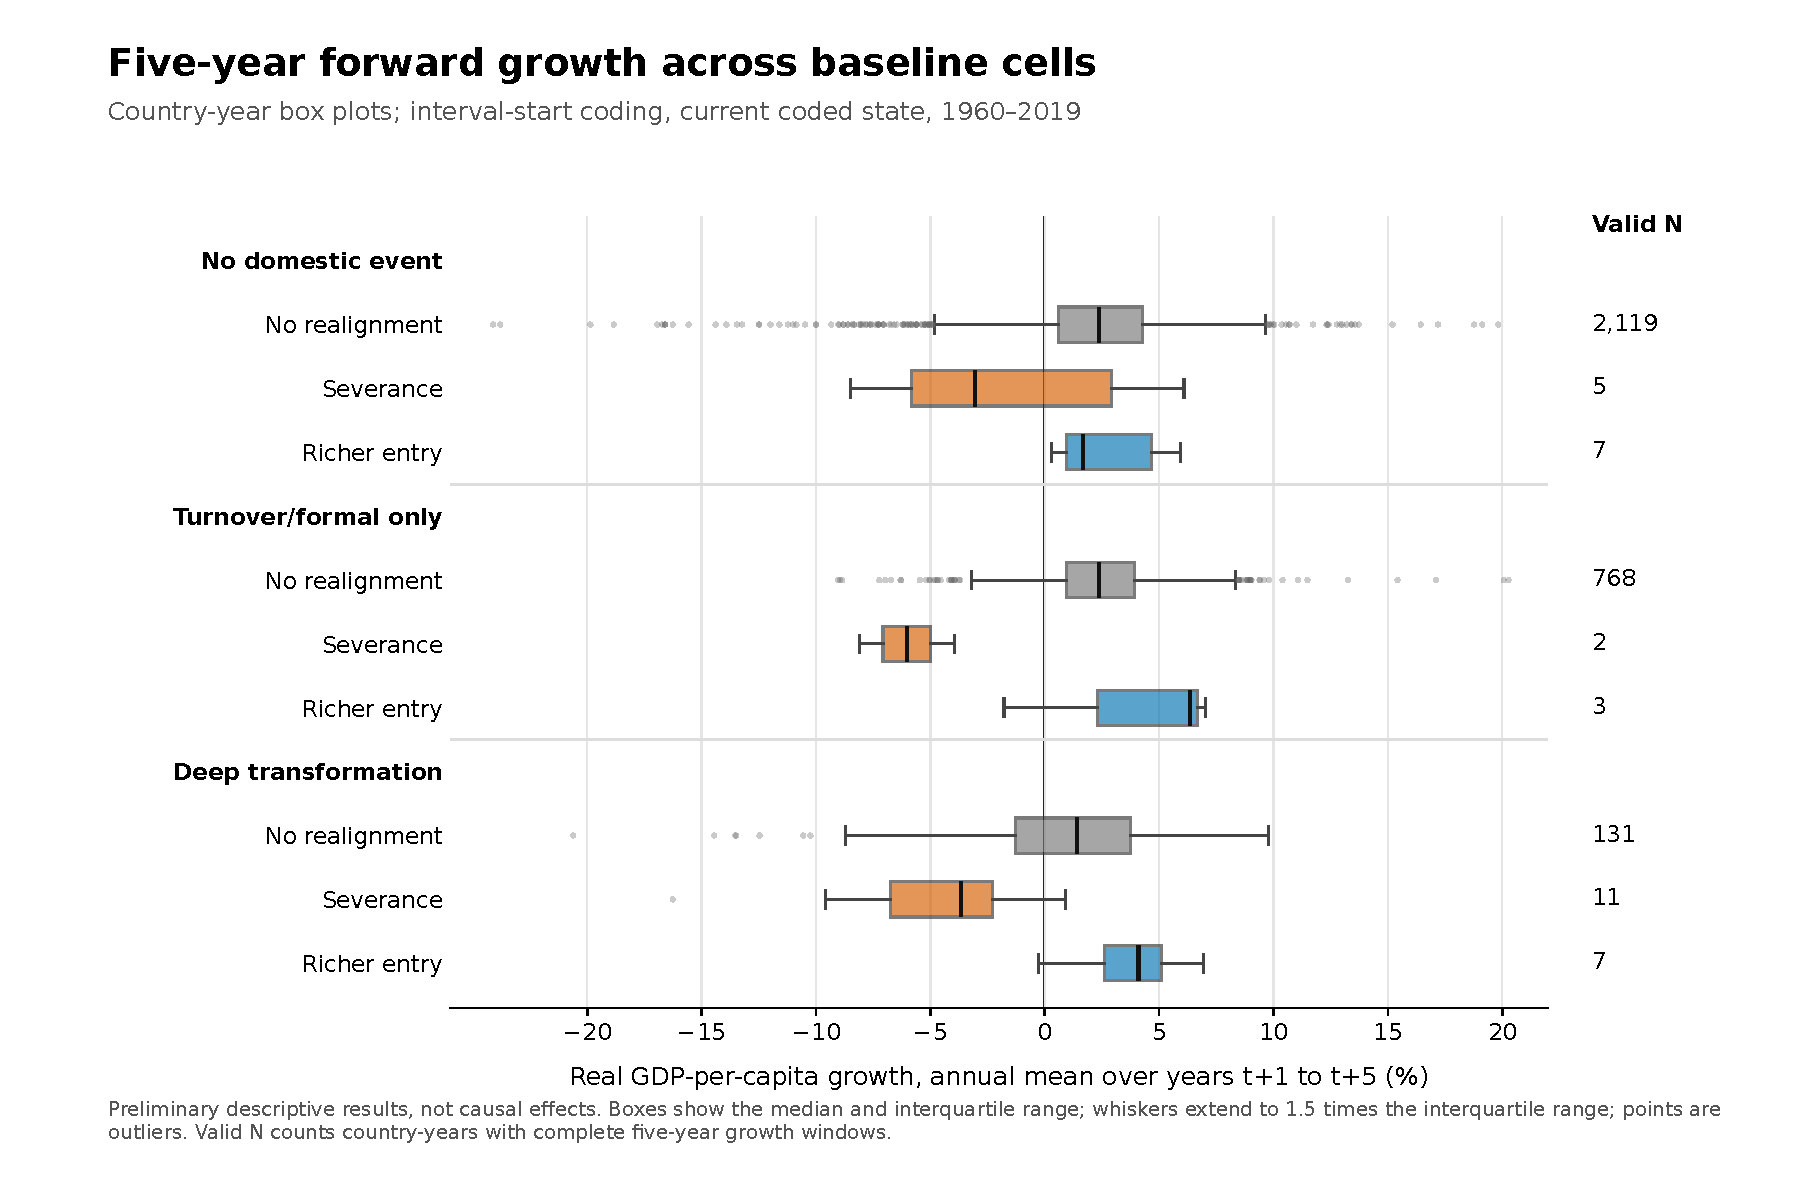
\includegraphics[width=\textwidth]{figures/step6_baseline_growth_boxplots_preliminary.pdf}
\caption{Distributions of five-year forward growth in the preliminary baseline cells.}
\label{fig:prelim_baseline_growth}
\end{figure}

\begin{figure}[htbp]
\centering
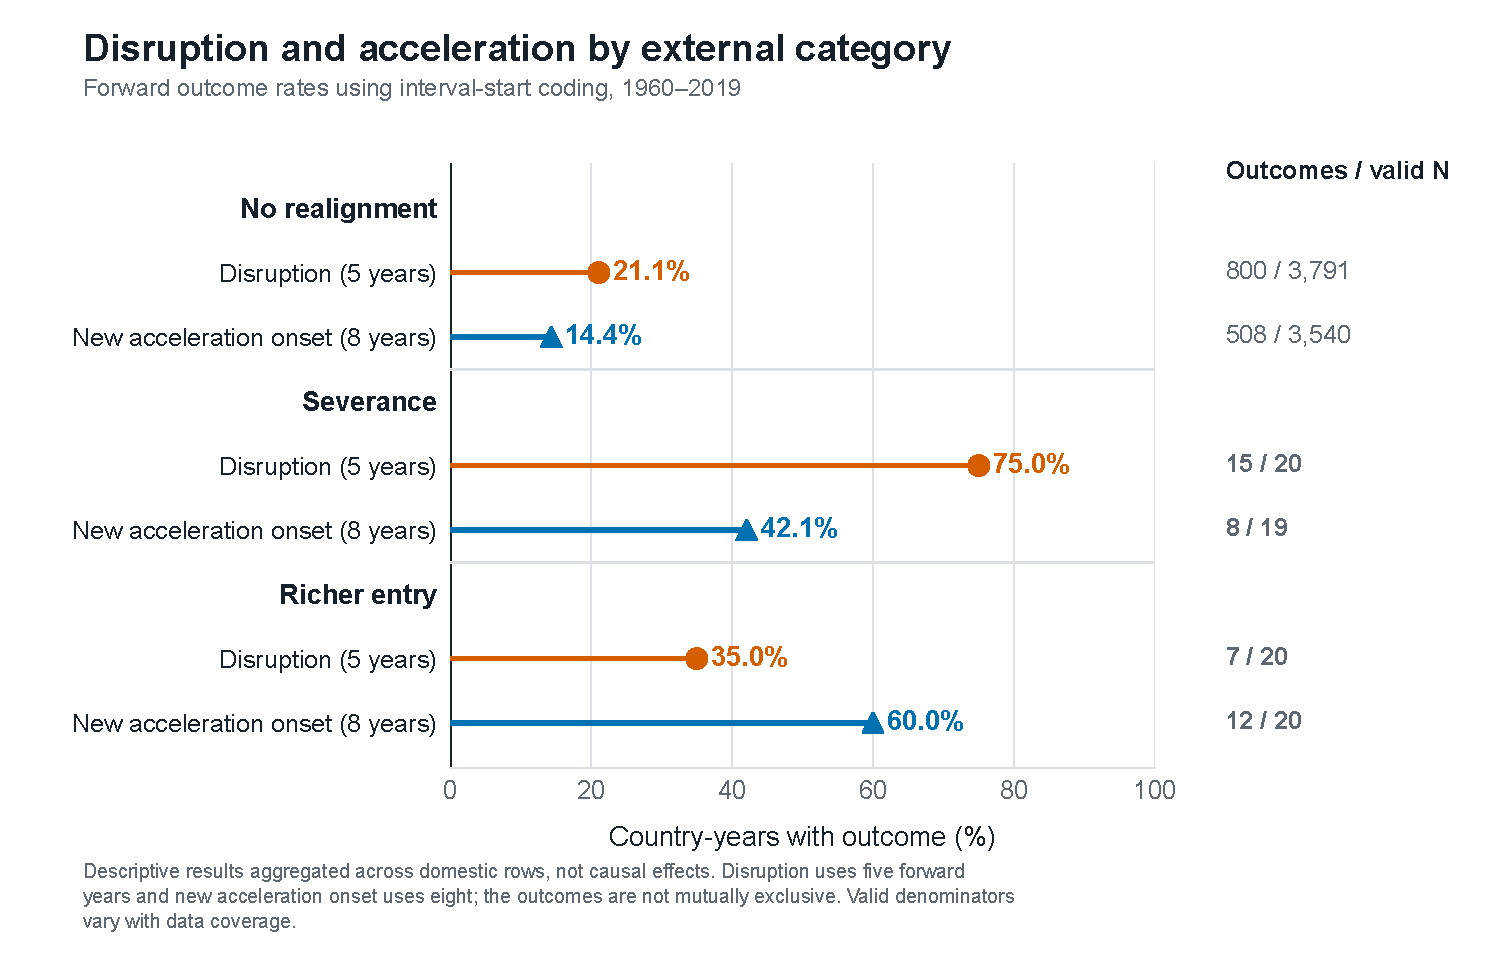
\includegraphics[width=\textwidth]{figures/step6_signed_outcomes_preliminary.pdf}
\caption{Forward disruption and acceleration by external category.}
\label{fig:prelim_signed_outcomes}
\end{figure}

\subsection{Timing and sensitivity}

The episode-level timing audit qualifies these aggregate contrasts. Twenty-three severance episodes and 23 richer-entry episodes fall inside the primary period under start-year coding. For each type, 14 have the signed outcome already active at the event and three are paired transitions. Among severances, two show disruption after the event and four show none in the registered window; among richer entries, three show a later acceleration onset and three show none. Cuba in 1989 and Venezuela in 2002, for example, already have active disruption, while Vietnam in 1994 already has an active acceleration. In these cases, the outcome predates the event and cannot be counted as a new consequence. The timing categories also warn against interpreting the country-year aggregates as clean episode-level treatment effects.

Table~\ref{tab:prelim_sensitivity} reports the principal date and case-selection sensitivities. Alternative dates change event timing and the classification of simultaneous episodes as paired, producing different observation counts. Severance mean growth rises from $-3.28$ percent at interval starts to $-0.16$ percent at midpoints and $+2.70$ percent at endpoints. Excluding open cases leaves a negative mean of $-2.59$ percent. After systemic-shift episodes are excluded, only five bare-severance observations remain, with positive mean growth of $+2.53$ percent. The six bare imposed-severance observations retain negative mean growth of $-3.29$ percent and an 83.3 percent disruption rate. This small, historically clustered subset cannot settle the causal claim.

Mean growth after richer entry remains positive under all three dating rules. By contrast, the new-acceleration rate falls from 60.0 percent at starts to 13.0 percent at midpoints and 13.6 percent at endpoints. Excluding open cases or systemic shifts preserves positive mean growth and higher start-date acceleration-onset rates; wrong-sign disruptions and the timing problem remain. Entry patterns depend on both the outcome measure and the dating convention.

\begin{table}[!ht]
\centering
\begin{threeparttable}
\caption{Preliminary aggregate sensitivities by external event}
\label{tab:prelim_sensitivity}
\small
\begin{tabular}{@{}p{0.27\linewidth}p{0.15\linewidth}rrrr@{}}
\toprule
Scenario & External category & $N$ & $\bar g_5$ (\%) & $D_5$ (\%) & $A_8$ (\%) \\
\midrule
Start, current coding & No realignment & 4,335 & 2.23 & 21.1 & 14.4 \\
Start, current coding & Severance & 20 & $-3.28$ & 75.0 & 42.1 \\
Midpoint, current coding & Severance & 23 & $-0.16$ & 72.7 & 63.6 \\
End, current coding & Severance & 23 & 2.70 & 61.9 & 66.7 \\
Start, excluding open cases & Severance & 19 & $-2.59$ & 73.7 & 38.9 \\
Start, excluding systemic shifts & Severance & 5 & 2.53 & 40.0 & 25.0 \\
Start, imposed severance only & Severance & 6 & $-3.29$ & 83.3 & 33.3 \\
\midrule
Start, current coding & Richer entry & 20 & 3.43 & 35.0 & 60.0 \\
Midpoint, current coding & Richer entry & 23 & 3.74 & 8.7 & 13.0 \\
End, current coding & Richer entry & 23 & 2.75 & 17.4 & 13.6 \\
Start, excluding open cases & Richer entry & 18 & 3.68 & 33.3 & 61.1 \\
Start, excluding systemic shifts & Richer entry & 16 & 3.37 & 31.3 & 50.0 \\
\bottomrule
\end{tabular}
\begin{tablenotes}
\small
\item Note: Preliminary, model-free descriptive results. Each external category aggregates domestic rows. $\bar g_5$ is mean real GDP-per-capita growth over five complete forward years. $D_5$ and $A_8$ are forward disruption and new acceleration-onset rates. Excluded event-years are removed from the sample and are never counted as no-realignment observations. Valid outcome denominators vary with coverage.
\end{tablenotes}
\end{threeparttable}
\end{table}

Figures~\ref{fig:prelim_sensitivity} and~\ref{fig:prelim_sensitivity_case_selection} show the growth distributions behind the means and the corresponding acceleration-onset rates. Growth boxes report medians and interquartile ranges, with whiskers at 1.5 times the interquartile range and points for outliers. Acceleration bars retain the onset rates, with event counts and valid denominators reported beside them. The five-year growth and eight-year acceleration windows have different coverage requirements, so their valid counts can differ.

\begin{figure}[!ht]
\centering
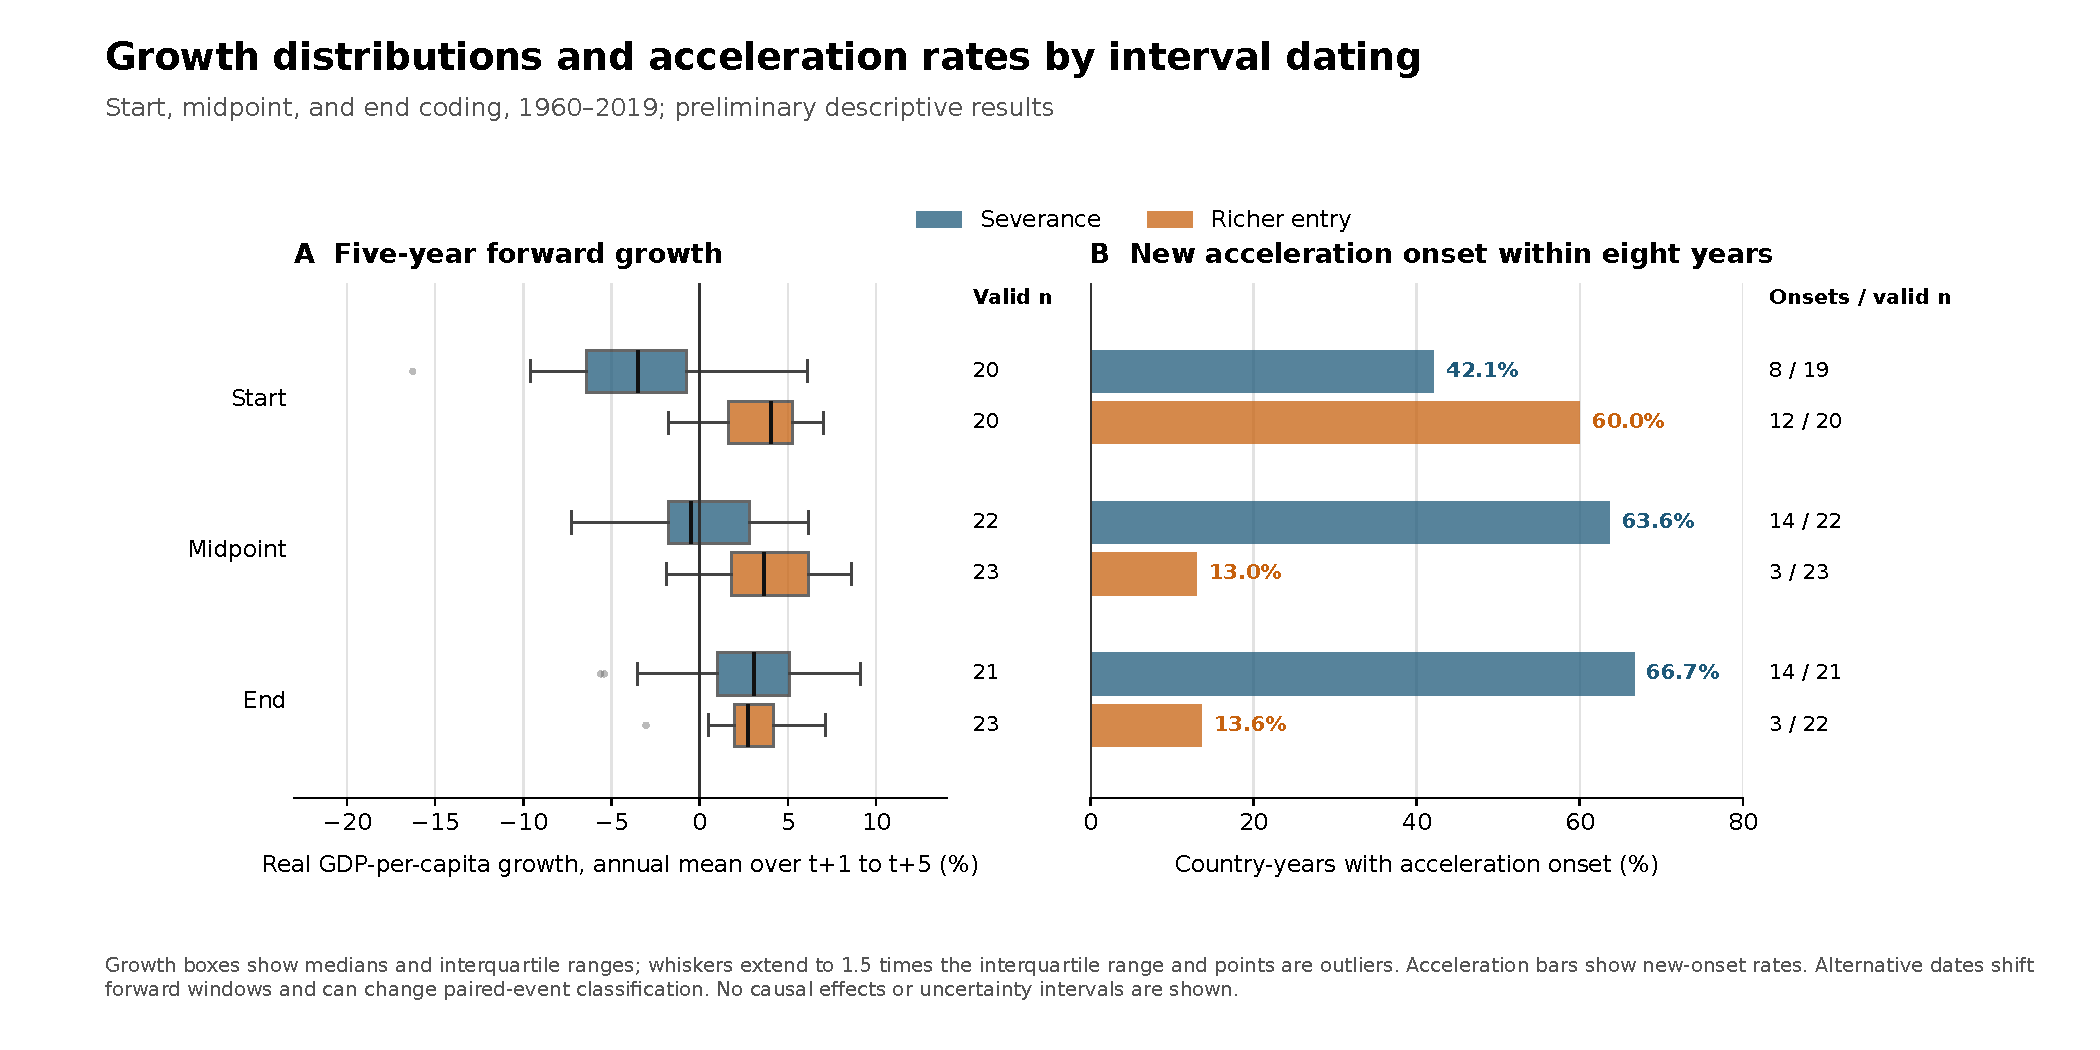
\includegraphics[width=\textwidth]{figures/step6_interval_dating_mixed_preliminary.pdf}
\caption{Five-year forward growth distributions and acceleration-onset rates by interval dating.}
\label{fig:prelim_sensitivity}
\end{figure}

\begin{figure}[!ht]
\centering
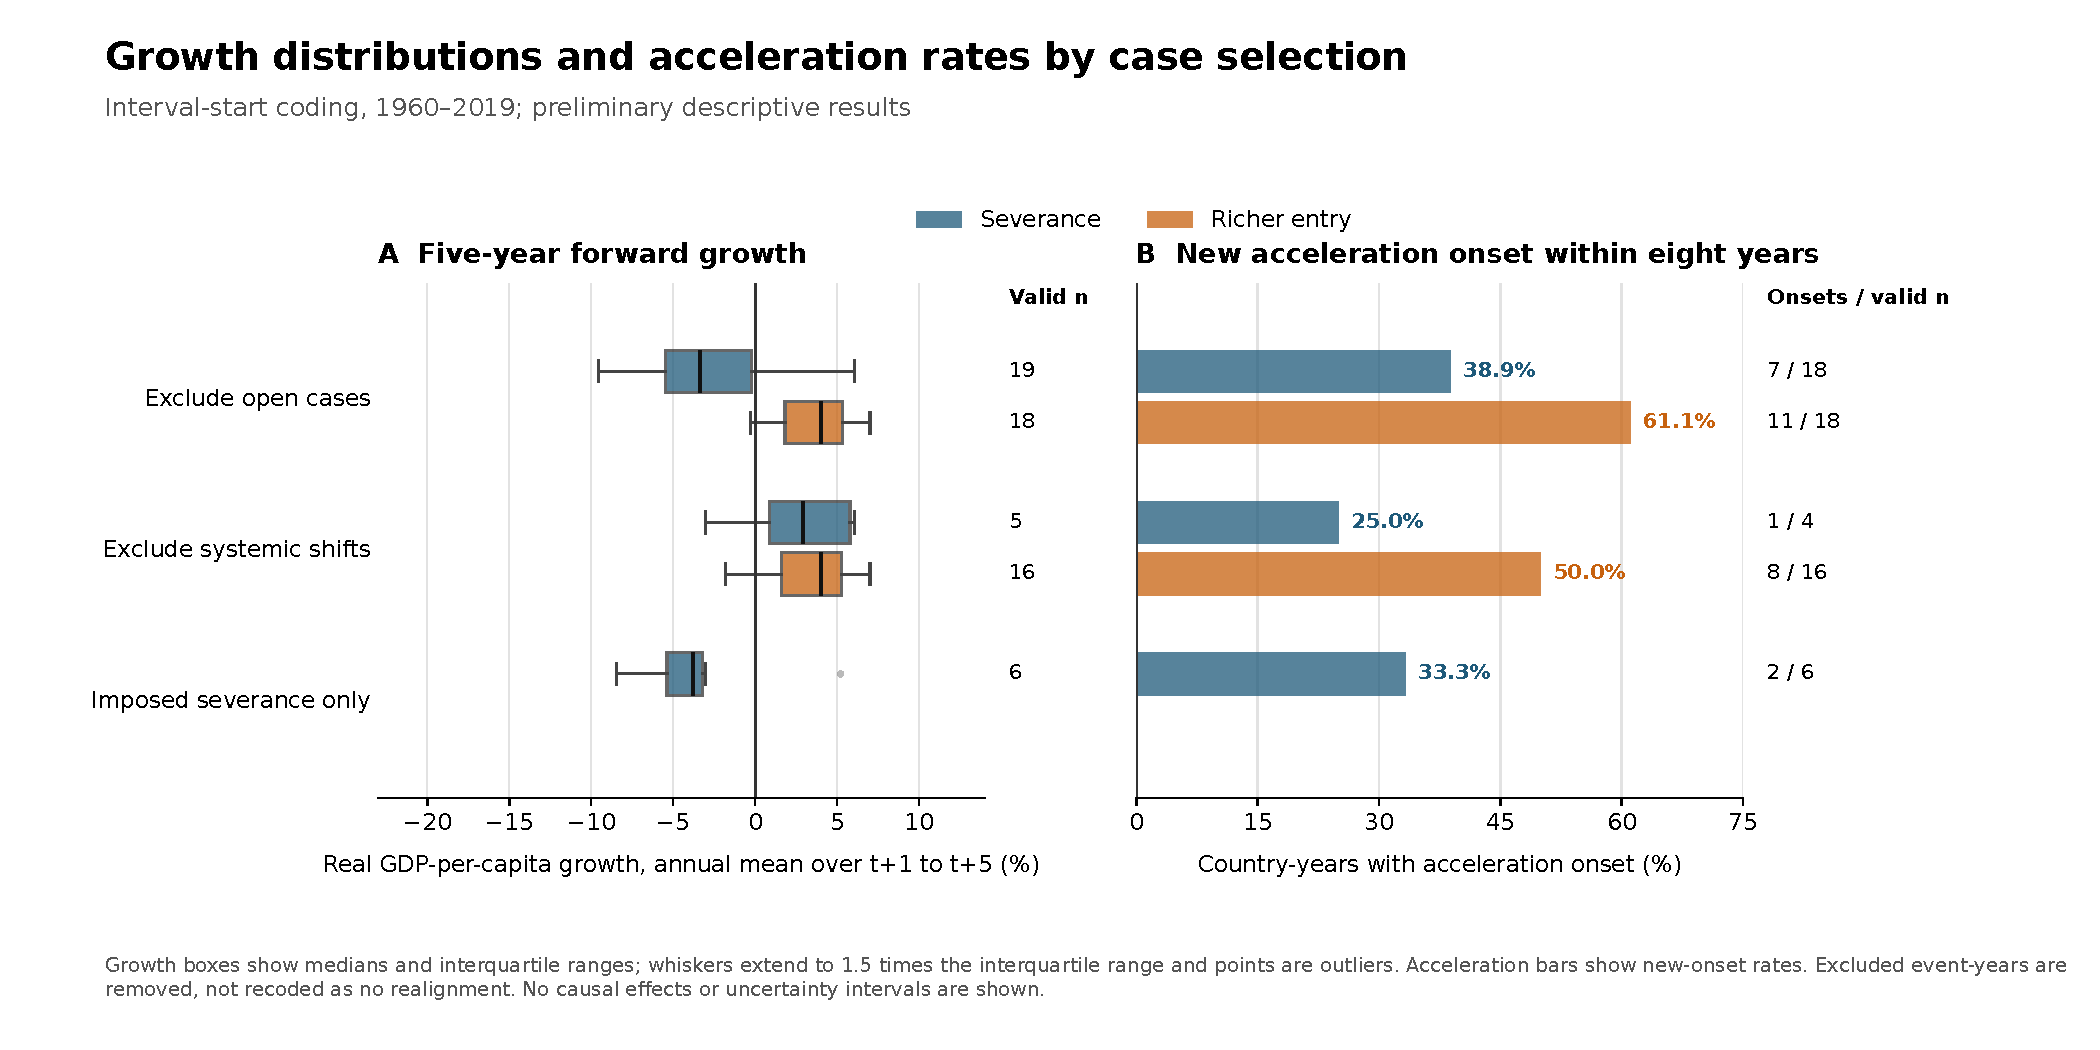
\includegraphics[width=\textwidth]{figures/step6_case_selection_mixed_preliminary.pdf}
\caption{Five-year forward growth distributions and acceleration-onset rates by case selection.}
\label{fig:prelim_sensitivity_case_selection}
\end{figure}

\subsection{Event-time growth profiles}

Figure~\ref{fig:event_time_all} displays annual outcomes around the 46 start-dated severance and richer-entry episodes in the primary sample, covering 28 countries. Where Table~\ref{tab:prelim_cells} summarizes complete forward windows, these profiles show each observed annual growth rate. The three panels extend three, five, and eight years in both directions from the event. Gray lines represent country-event trajectories at 0.5 opacity; black lines are equally weighted means of the episodes observed at each event year. Missing observations interrupt the gray lines and can change the composition of the black mean. Severance and richer entry remain separate because $H_2$ assigns them opposite signs.

The profiles describe event-time patterns and provide no causal event-study estimates. Pre-event outcomes, ongoing outcomes, and paired transitions remain visible without any implication that the event initiated them. Figures~\ref{fig:event_time_hispanic_america}--\ref{fig:event_time_eastern_europe} divide the episodes among mutually exclusive cultural groups for visual presentation. These provisional groups draw on broad linguistic, historical, and regional-cultural context. They play no role in analytical coding and cannot establish cultural moderation of the material mechanisms in Section~\ref{sec:framework}. Groups without eligible realignments are omitted. Central Asia and Eastern Europe each contain one episode; in those panels, the black line is a single country's trajectory and involves no regional averaging.

\begin{figure}[p]
\centering
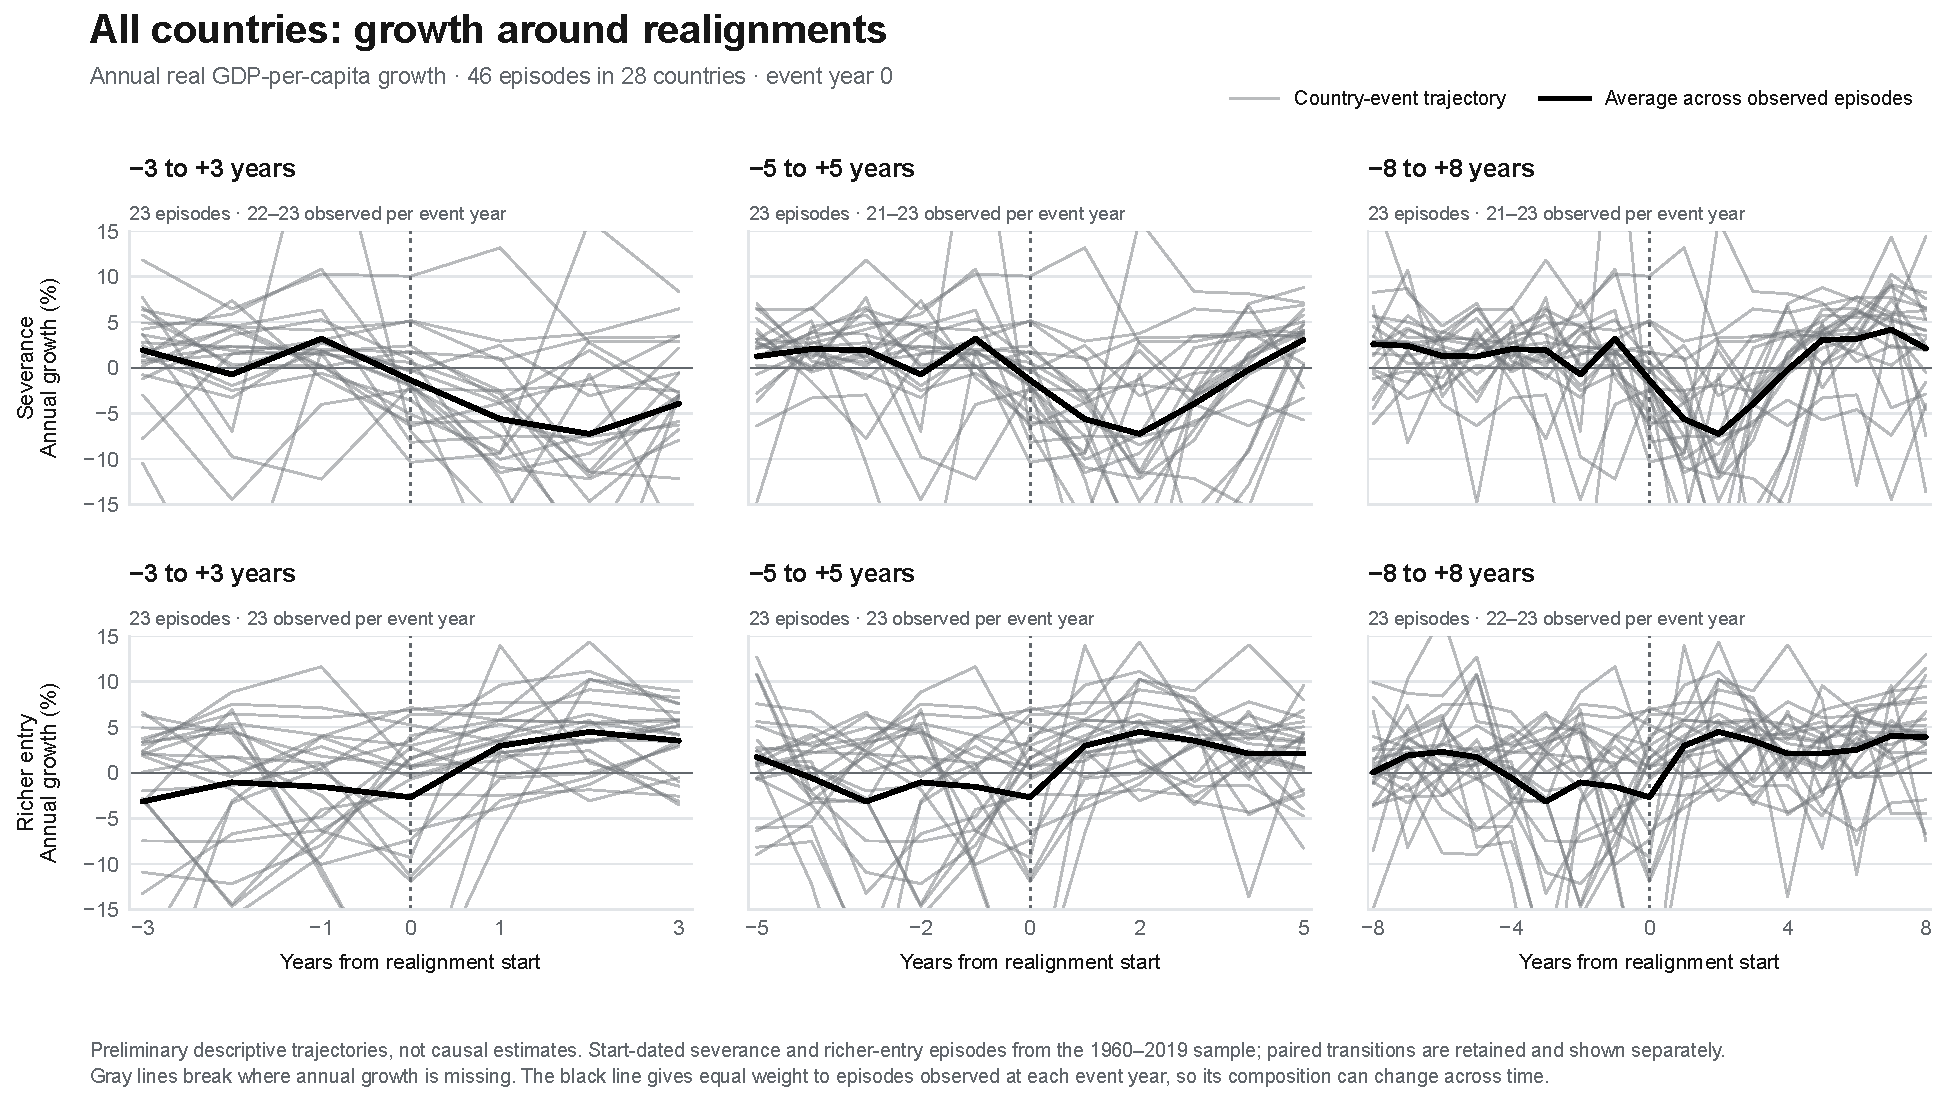
\includegraphics[width=\textwidth]{figures/event_time/all_countries_event_time_preliminary.pdf}
\caption{Annual real GDP-per-capita growth around 46 realignment episodes in 28 countries, 1960--2019.}
\label{fig:event_time_all}
\end{figure}

\begin{figure}[p]
\centering
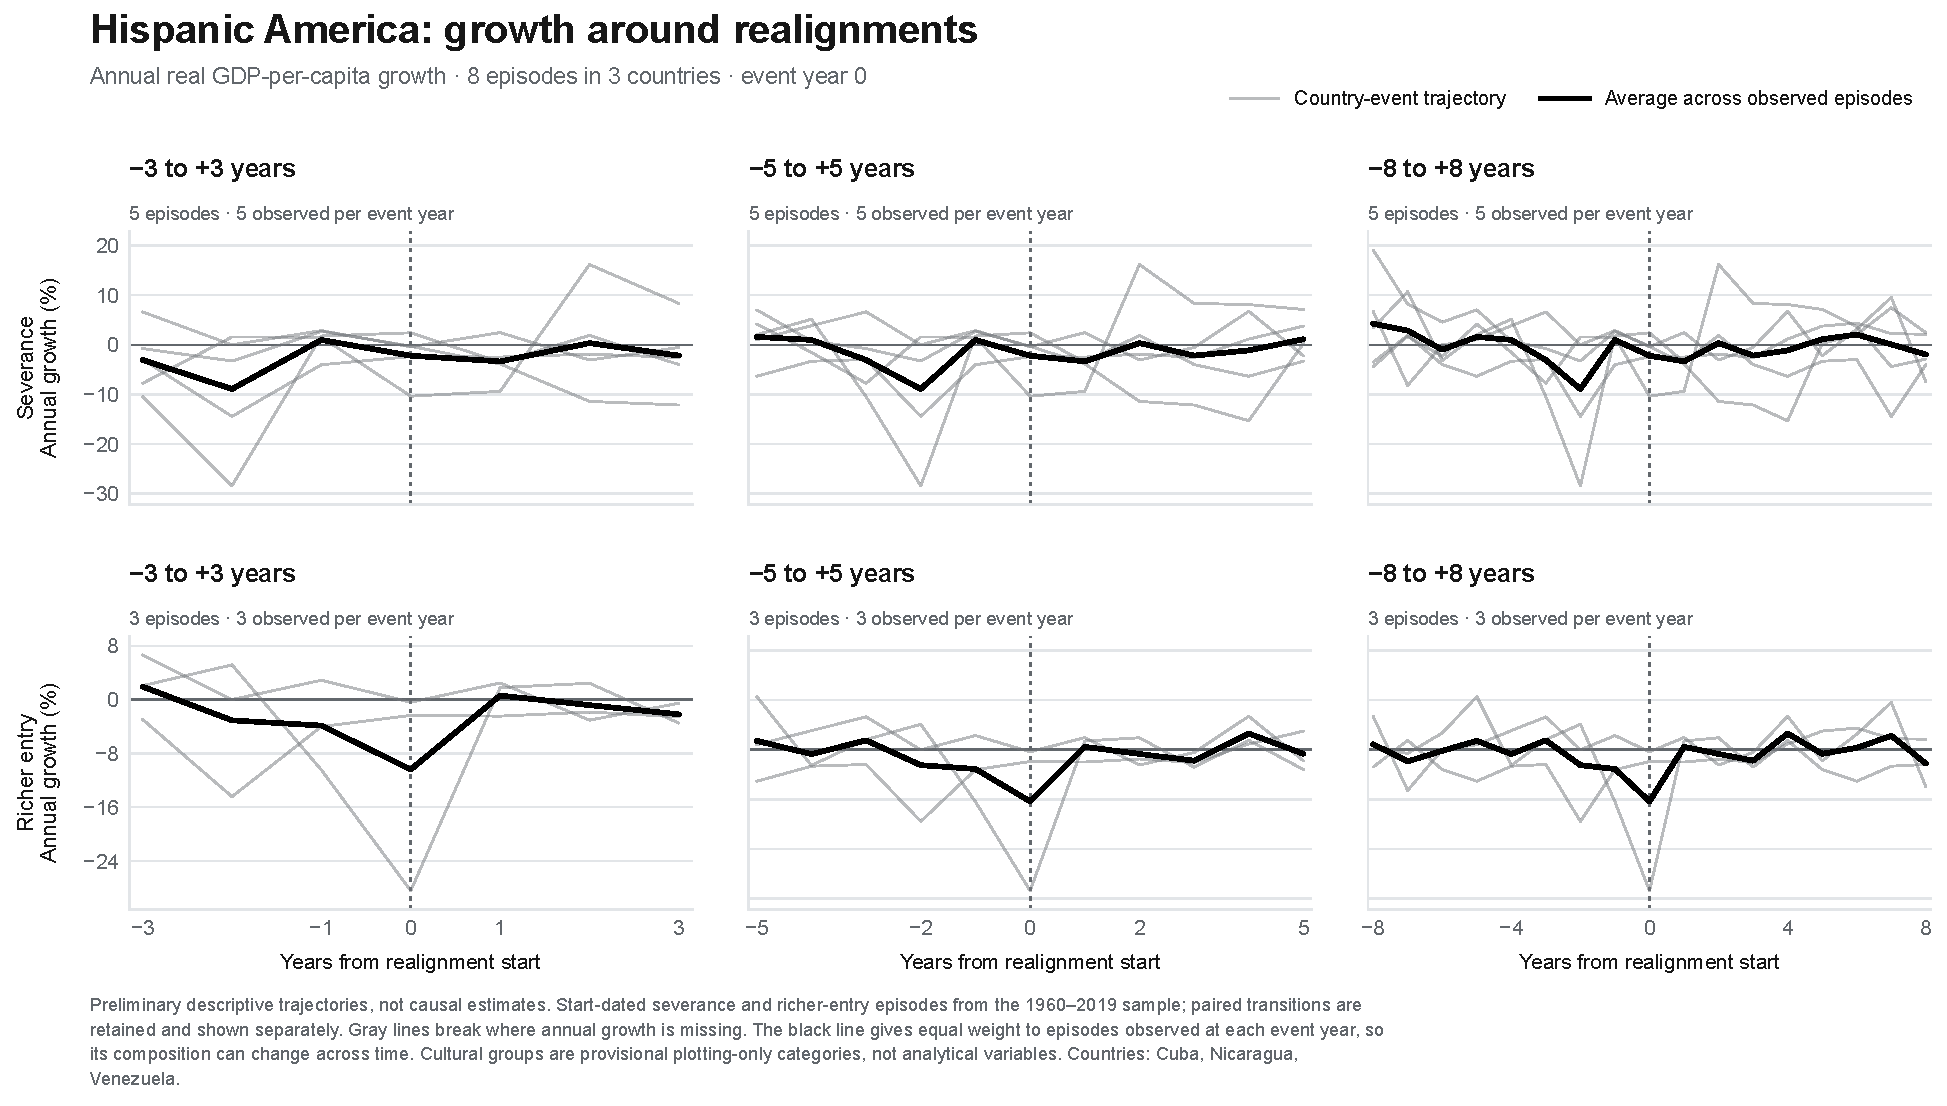
\includegraphics[width=\textwidth]{figures/event_time/hispanic_america_event_time_preliminary.pdf}
\caption{Event-time growth profiles: Hispanic America.}
\label{fig:event_time_hispanic_america}
\end{figure}

\begin{figure}[p]
\centering
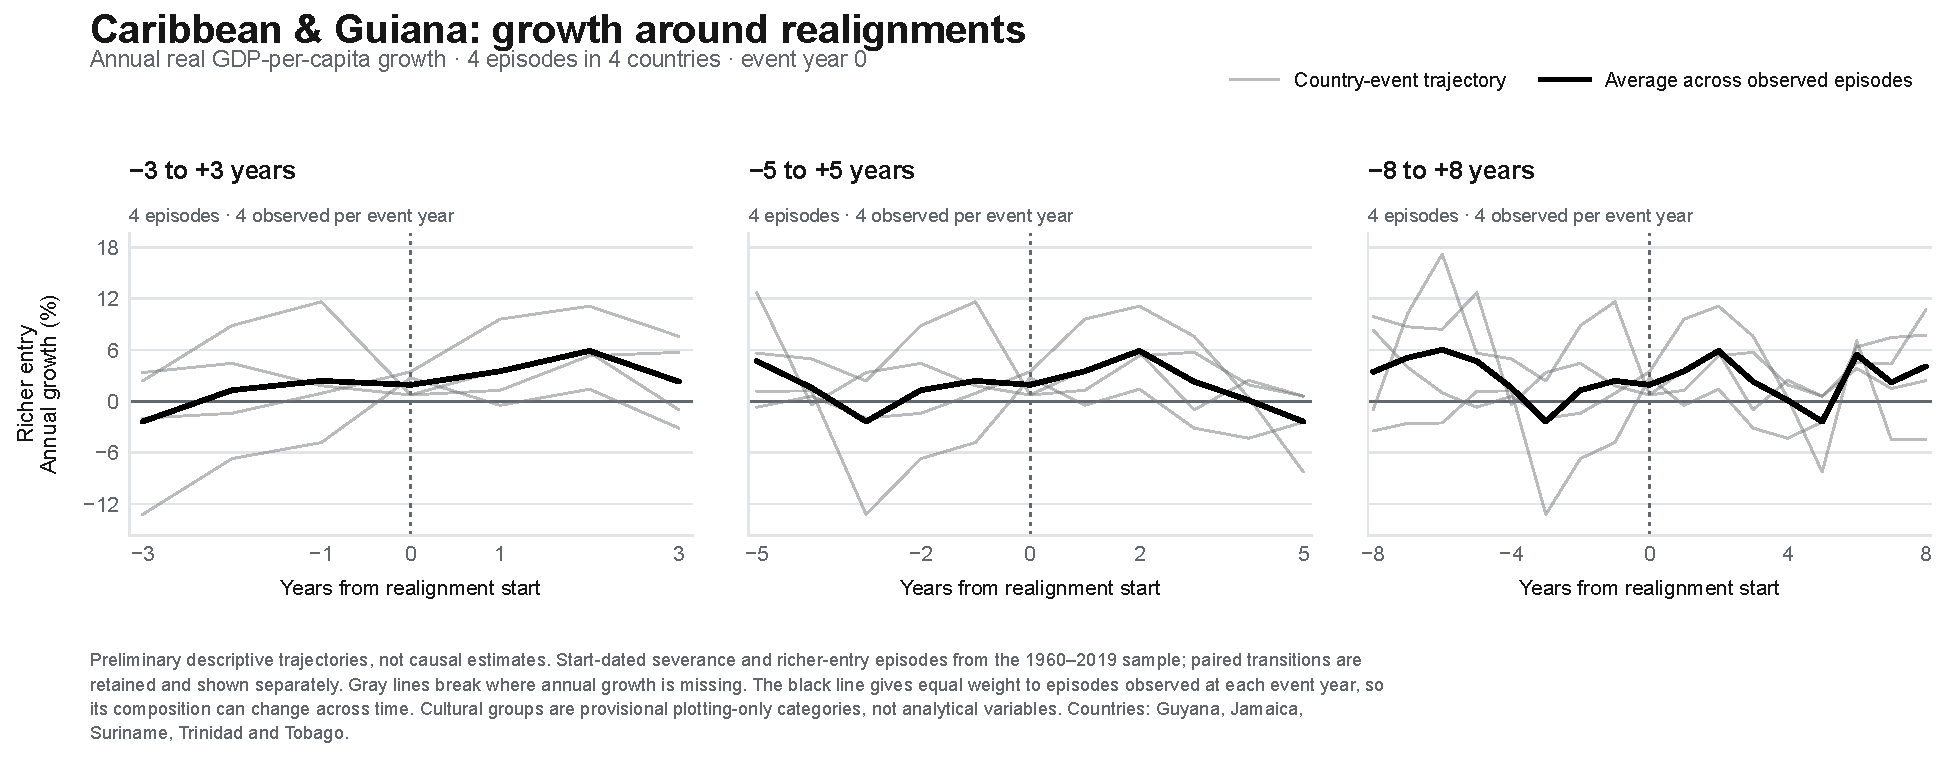
\includegraphics[width=\textwidth]{figures/event_time/caribbean_guiana_event_time_preliminary.pdf}
\caption{Event-time growth profiles: Caribbean and Guiana.}
\label{fig:event_time_caribbean_guiana}
\end{figure}

\begin{figure}[p]
\centering
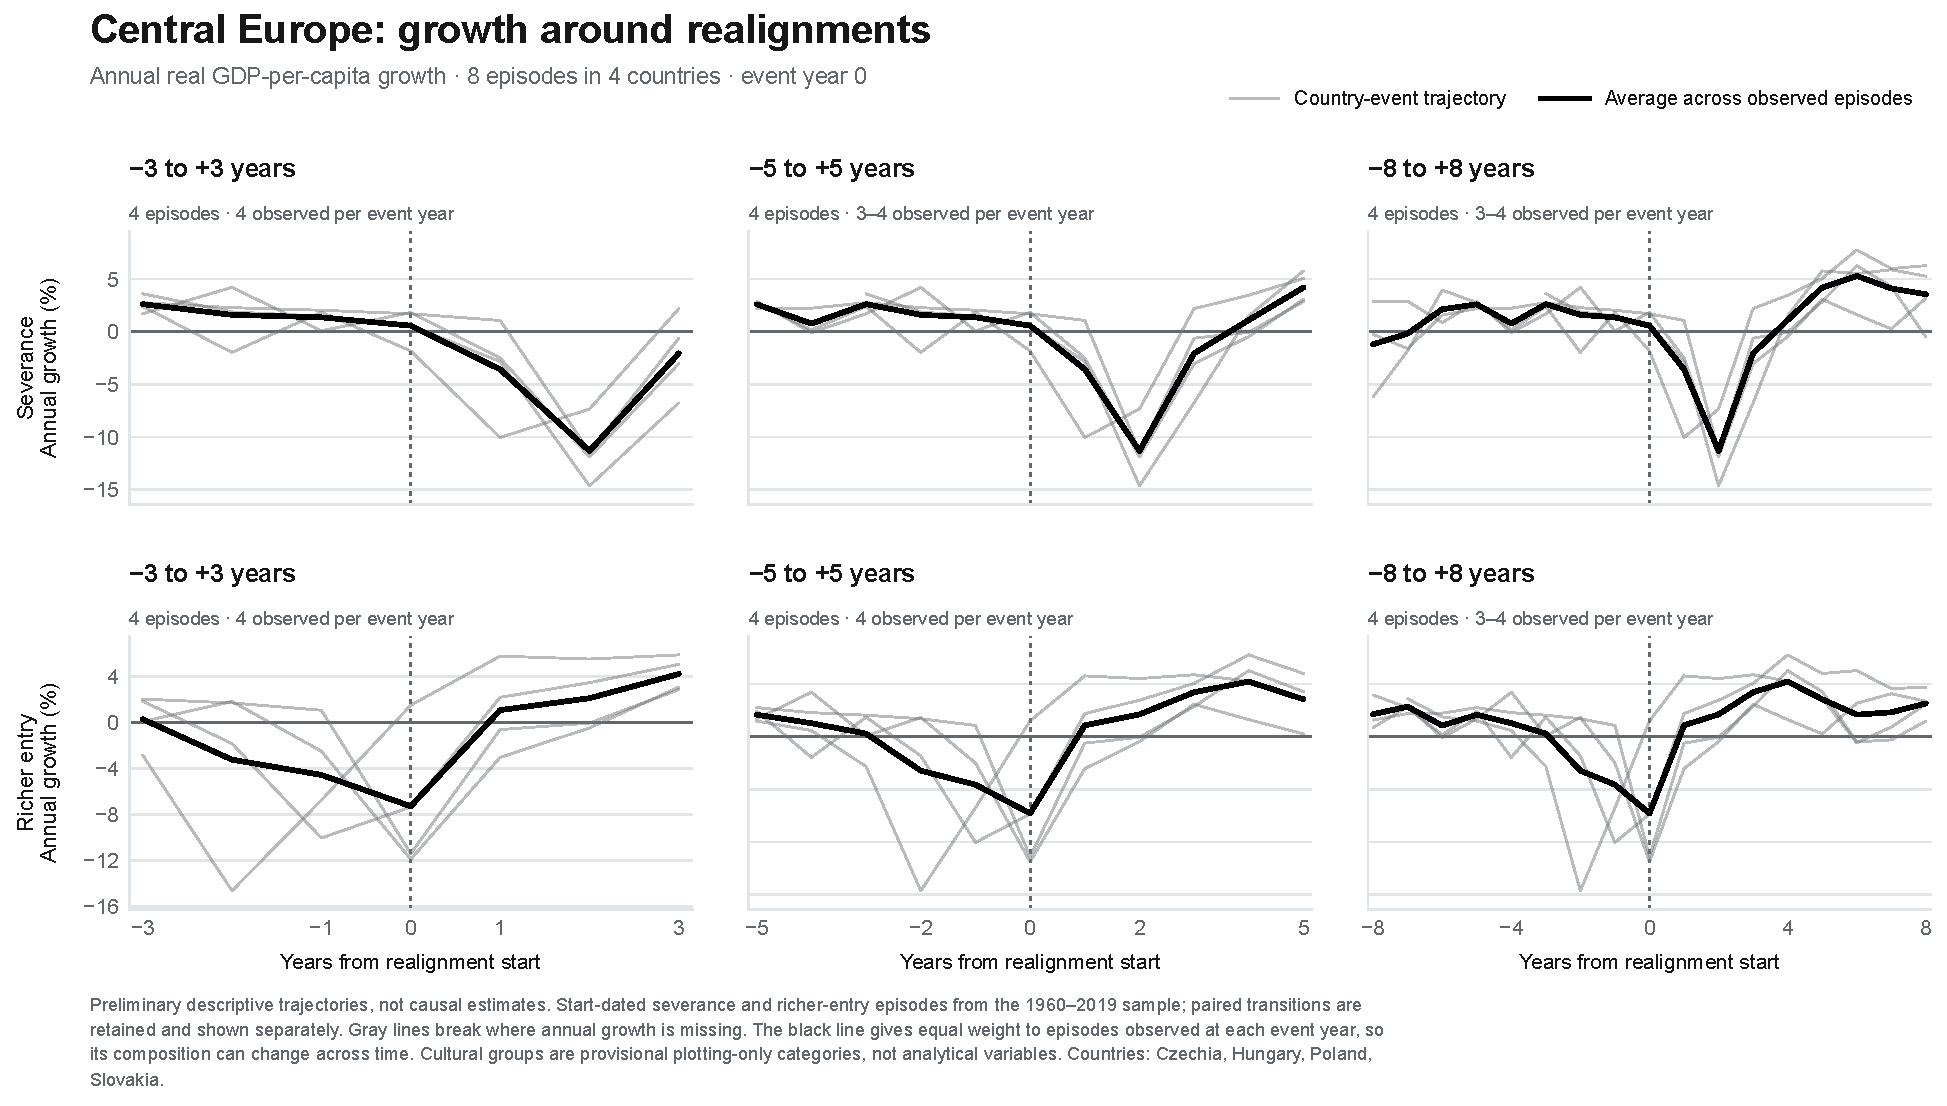
\includegraphics[width=\textwidth]{figures/event_time/central_europe_event_time_preliminary.pdf}
\caption{Event-time growth profiles: Central Europe.}
\label{fig:event_time_central_europe}
\end{figure}

\begin{figure}[p]
\centering
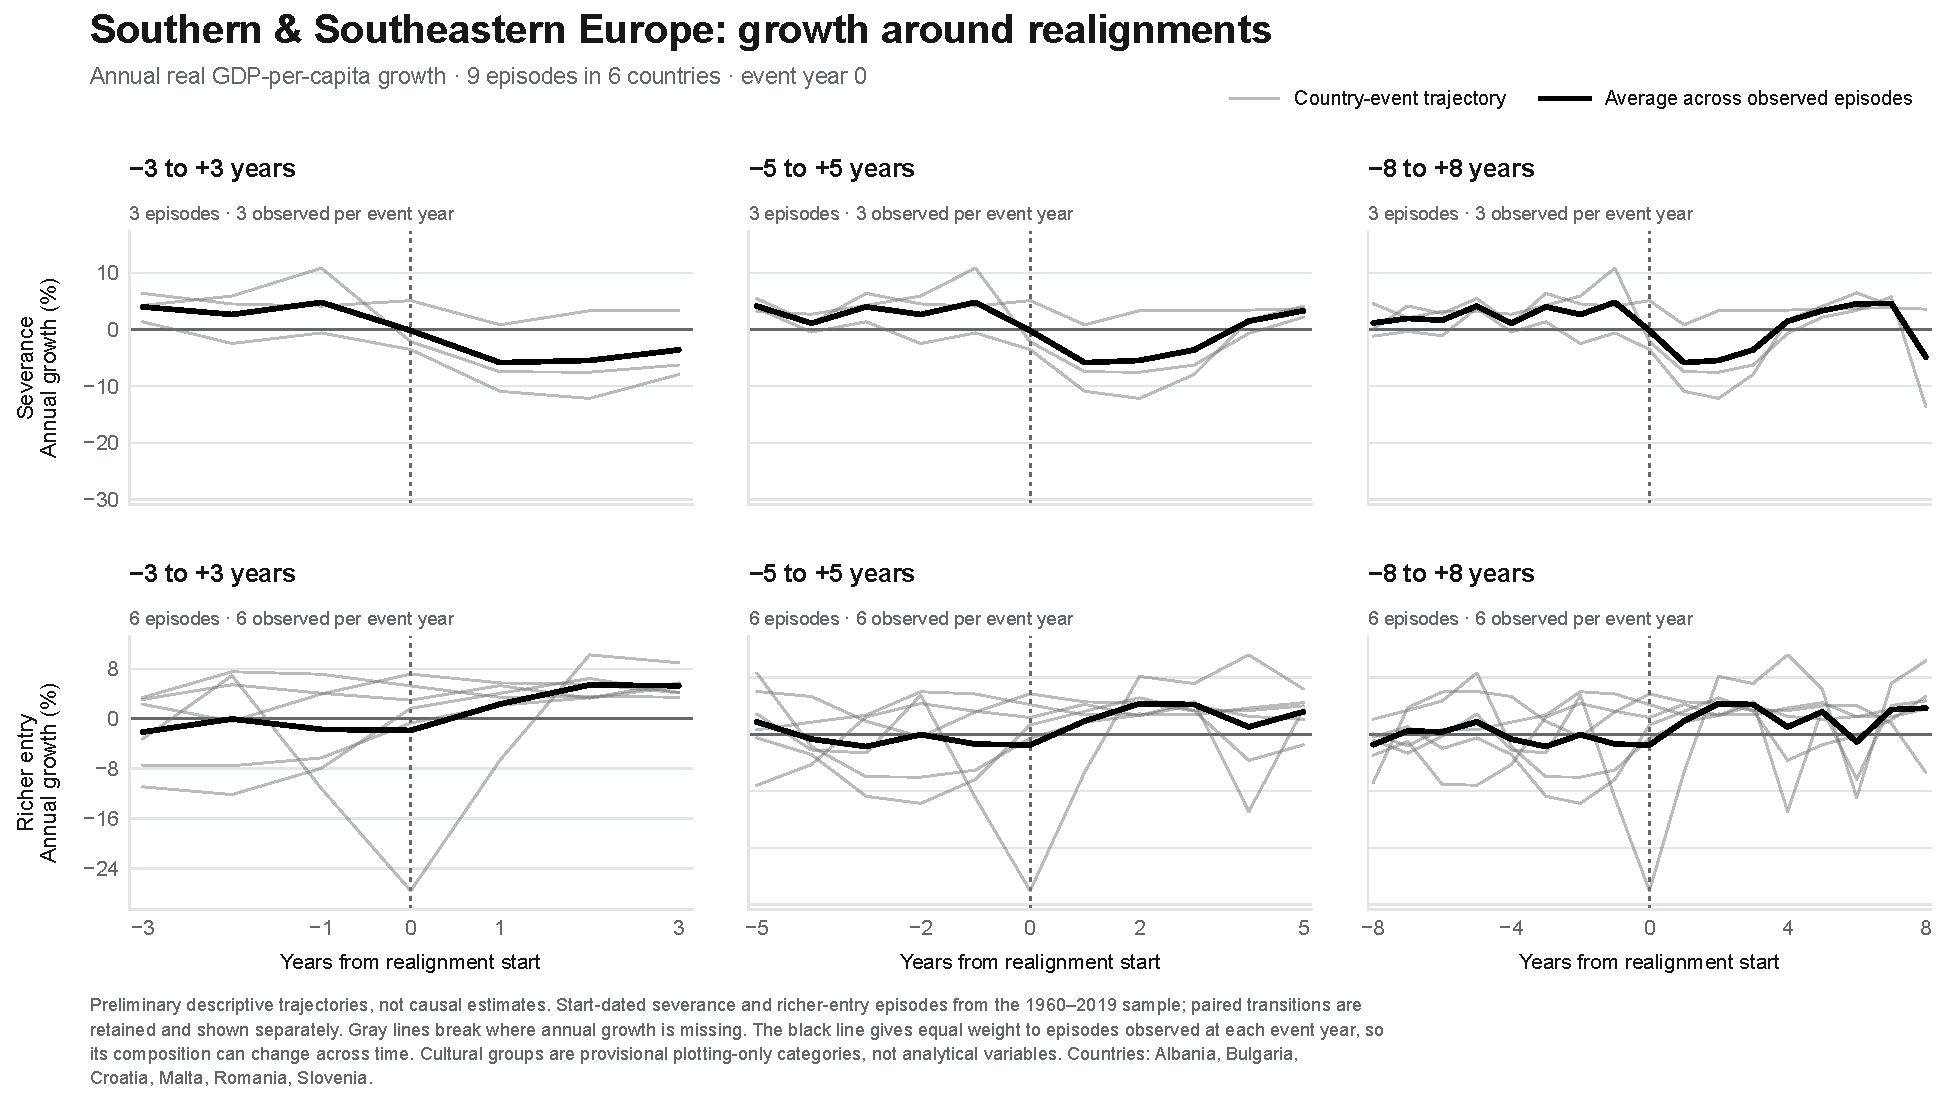
\includegraphics[width=\textwidth]{figures/event_time/southern_southeastern_europe_event_time_preliminary.pdf}
\caption{Event-time growth profiles: Southern and Southeastern Europe.}
\label{fig:event_time_southern_southeastern_europe}
\end{figure}

\begin{figure}[p]
\centering
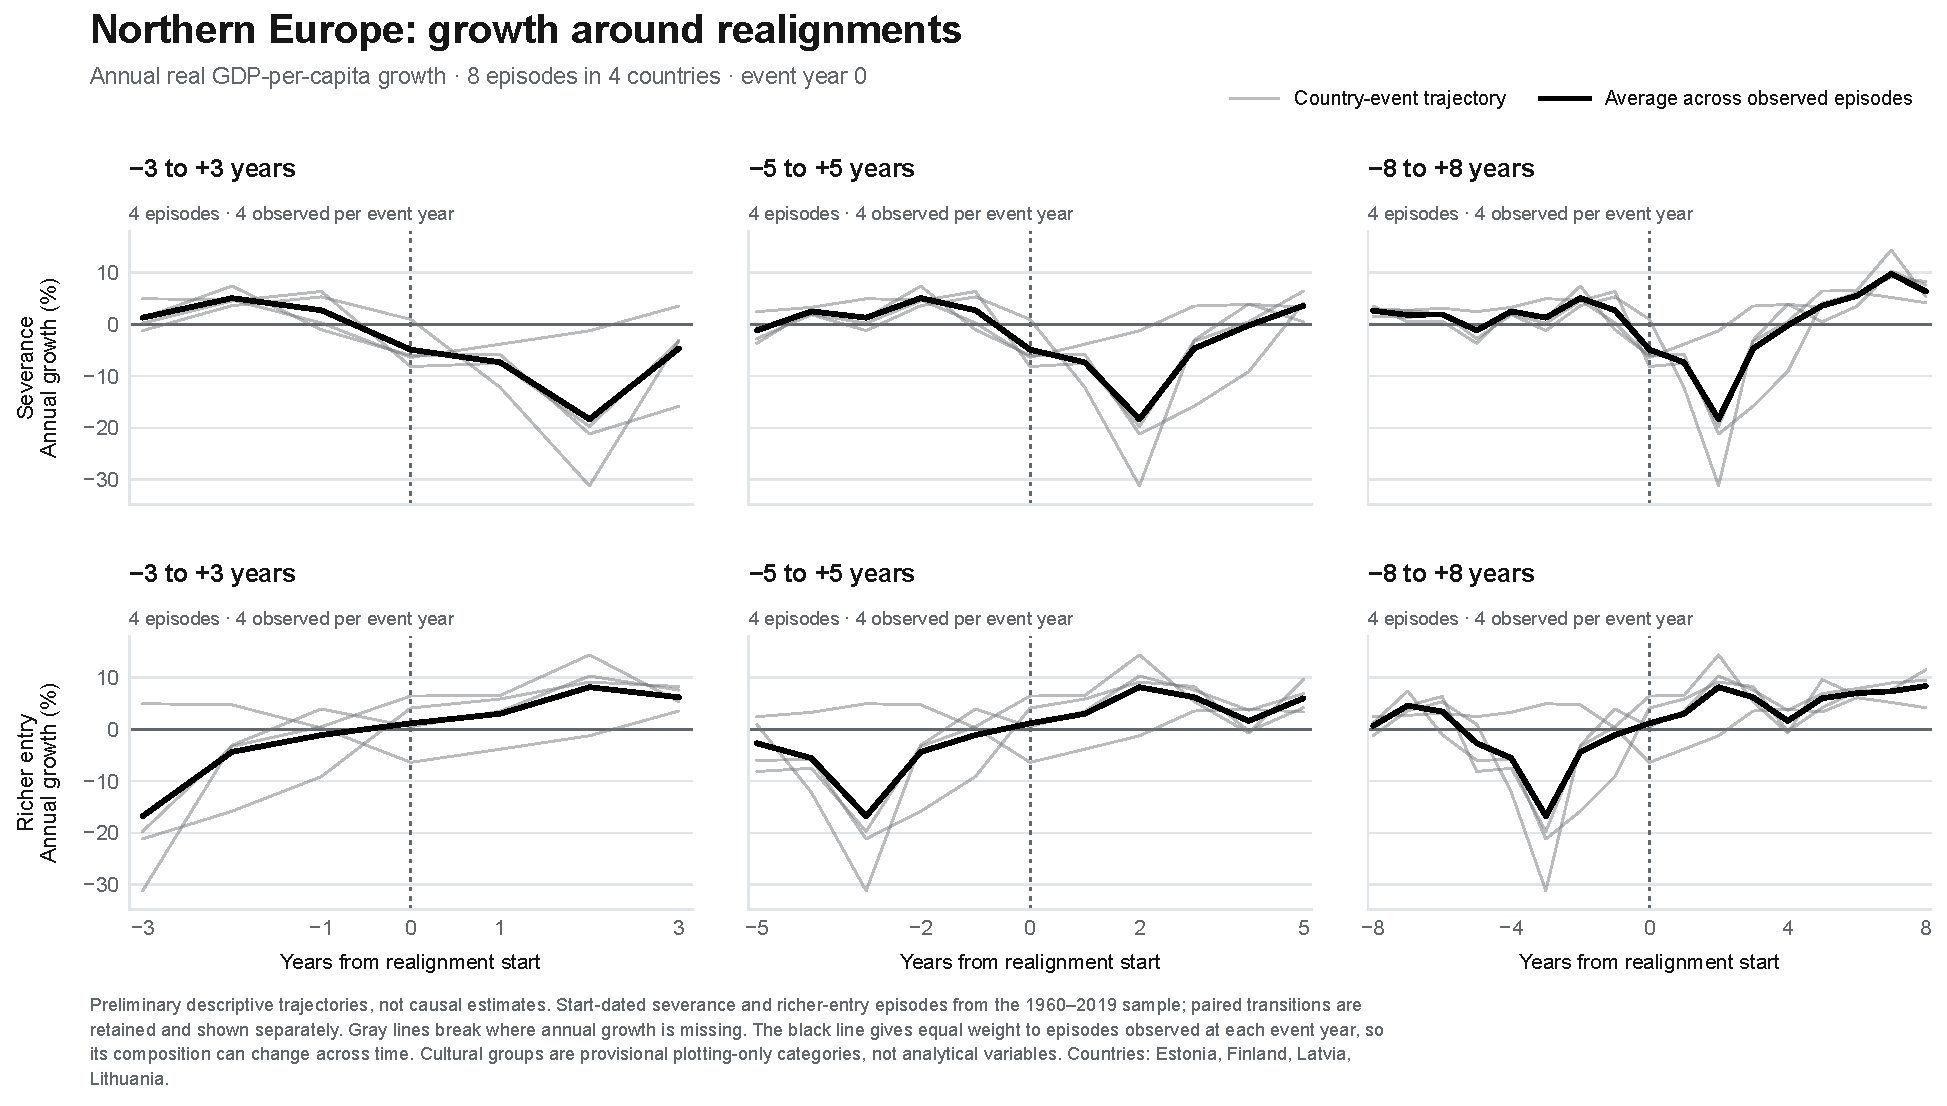
\includegraphics[width=\textwidth]{figures/event_time/northern_europe_event_time_preliminary.pdf}
\caption{Event-time growth profiles: Northern Europe.}
\label{fig:event_time_northern_europe}
\end{figure}

\begin{figure}[p]
\centering
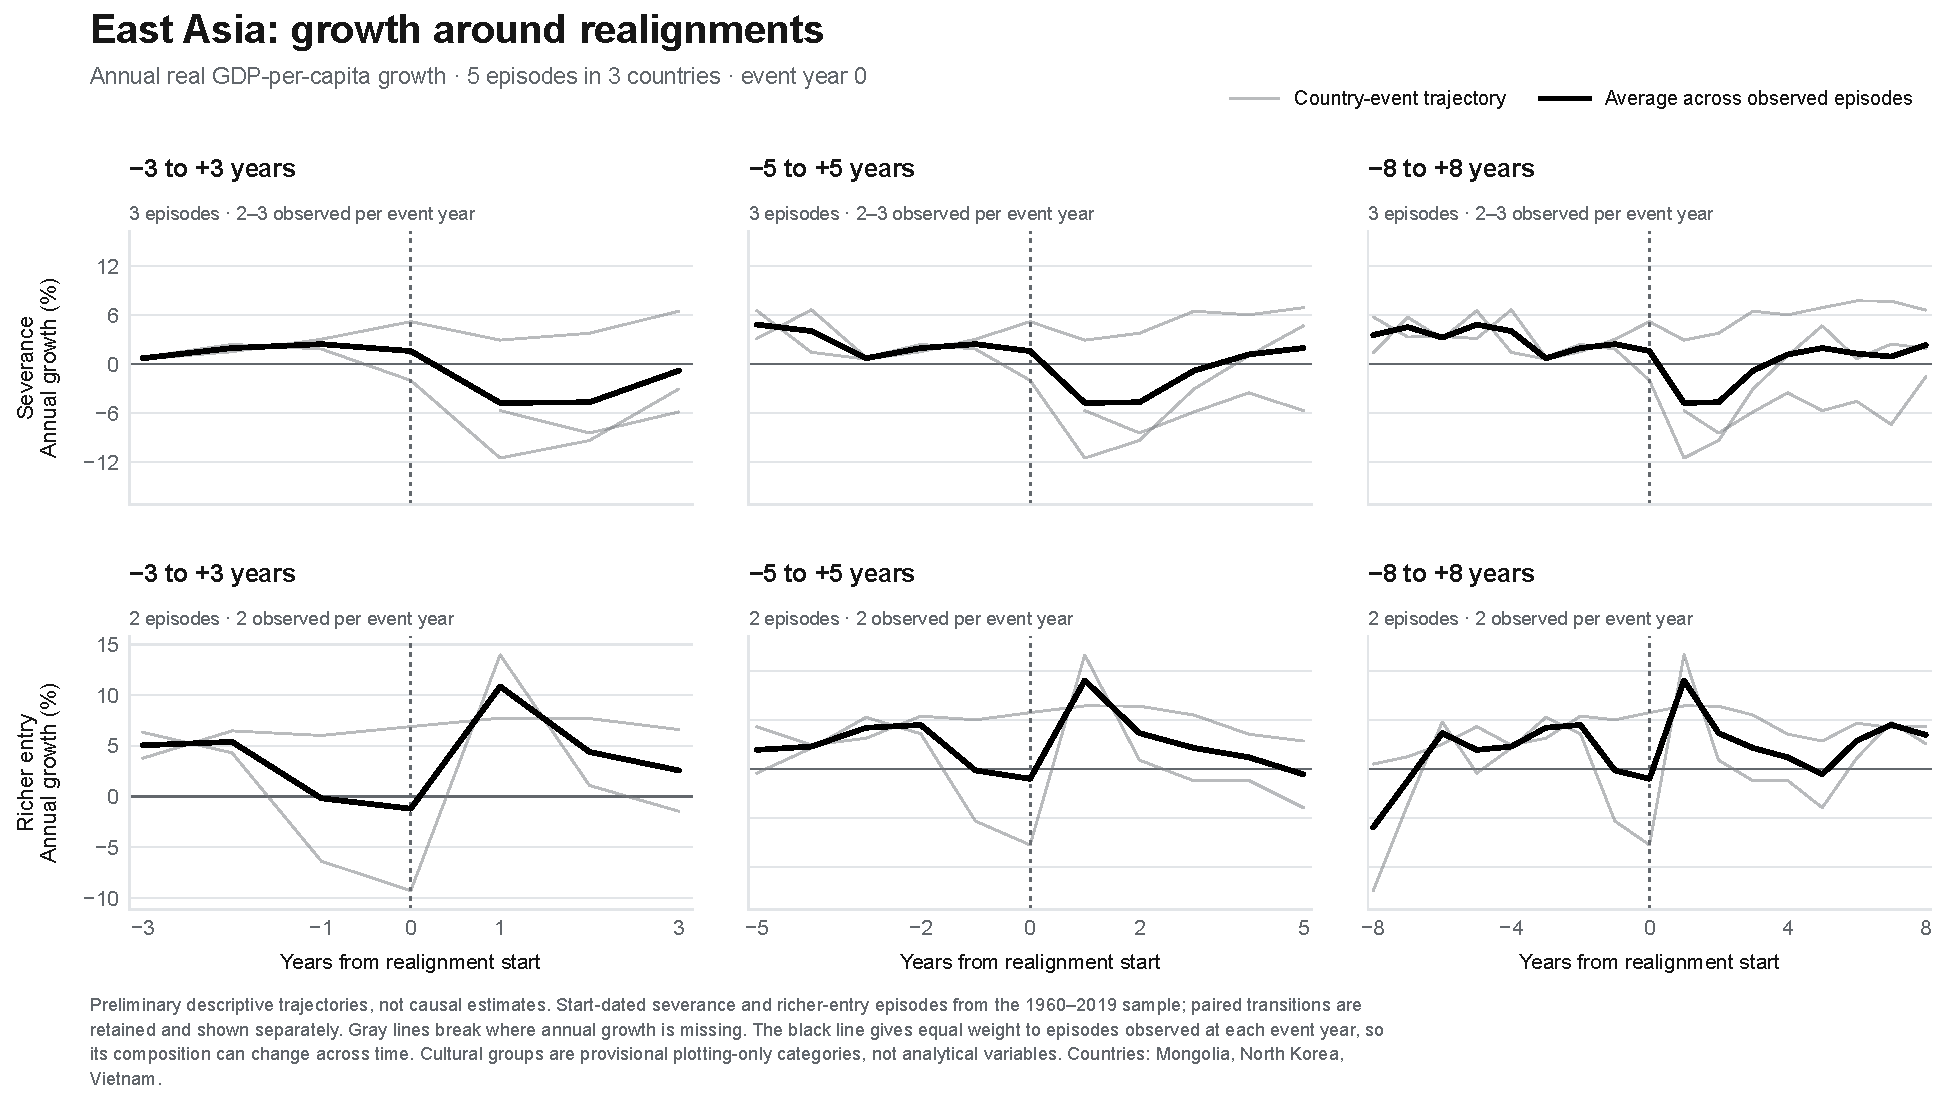
\includegraphics[width=\textwidth]{figures/event_time/east_asia_event_time_preliminary.pdf}
\caption{Event-time growth profiles: East Asia.}
\label{fig:event_time_east_asia}
\end{figure}

\begin{figure}[p]
\centering
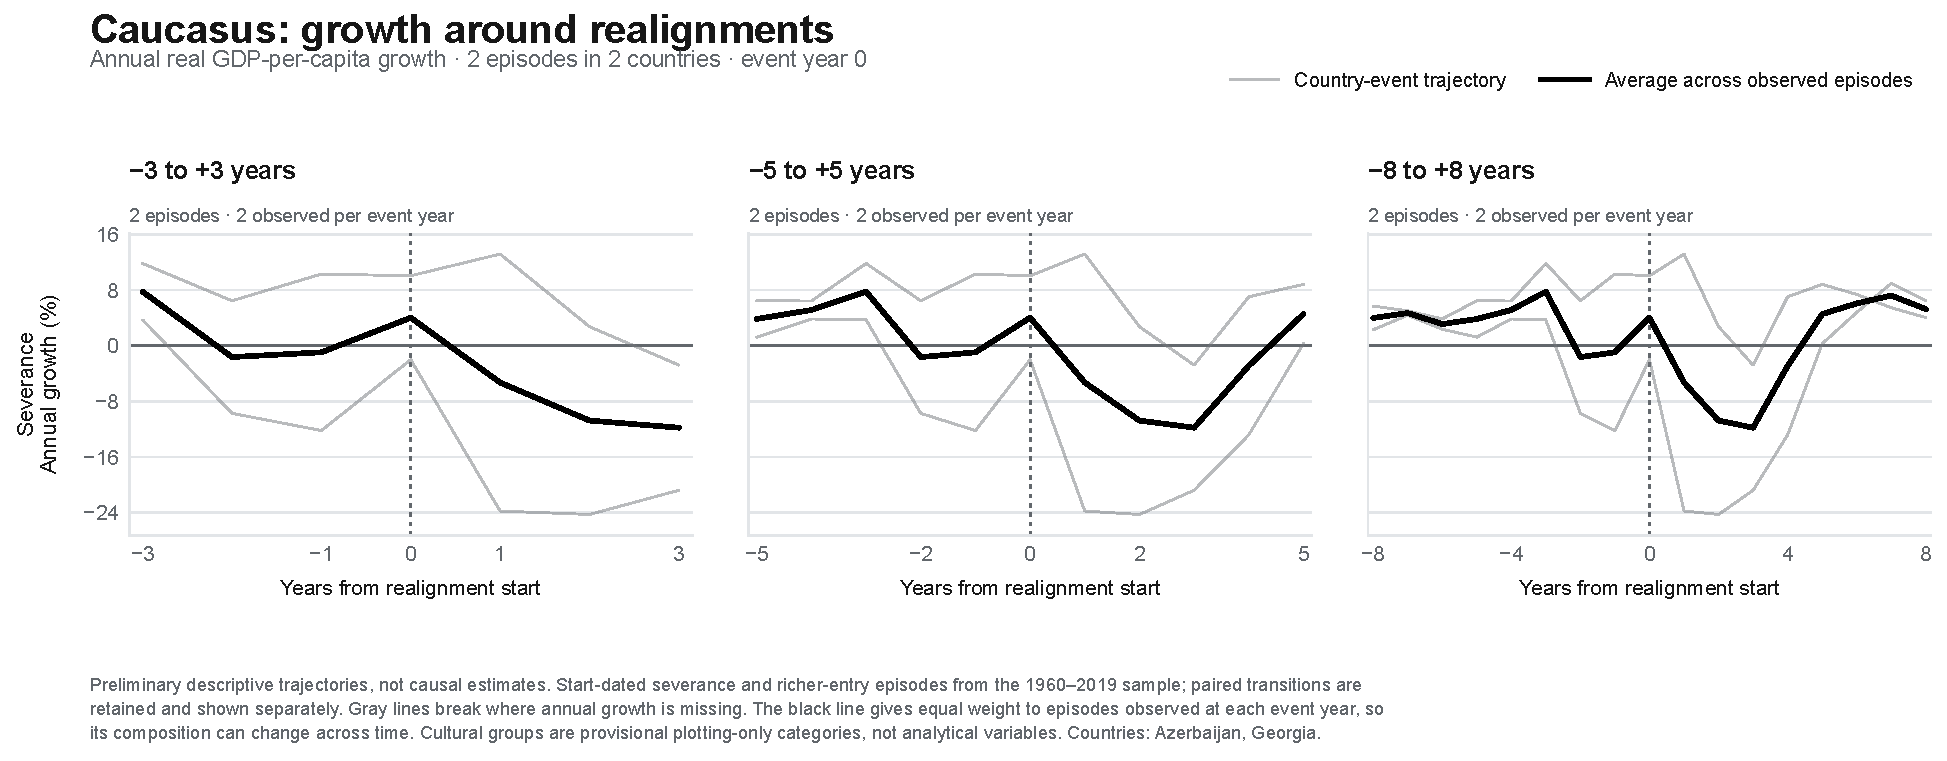
\includegraphics[width=\textwidth]{figures/event_time/caucasus_event_time_preliminary.pdf}
\caption{Event-time growth profiles: the Caucasus.}
\label{fig:event_time_caucasus}
\end{figure}

\begin{figure}[p]
\centering
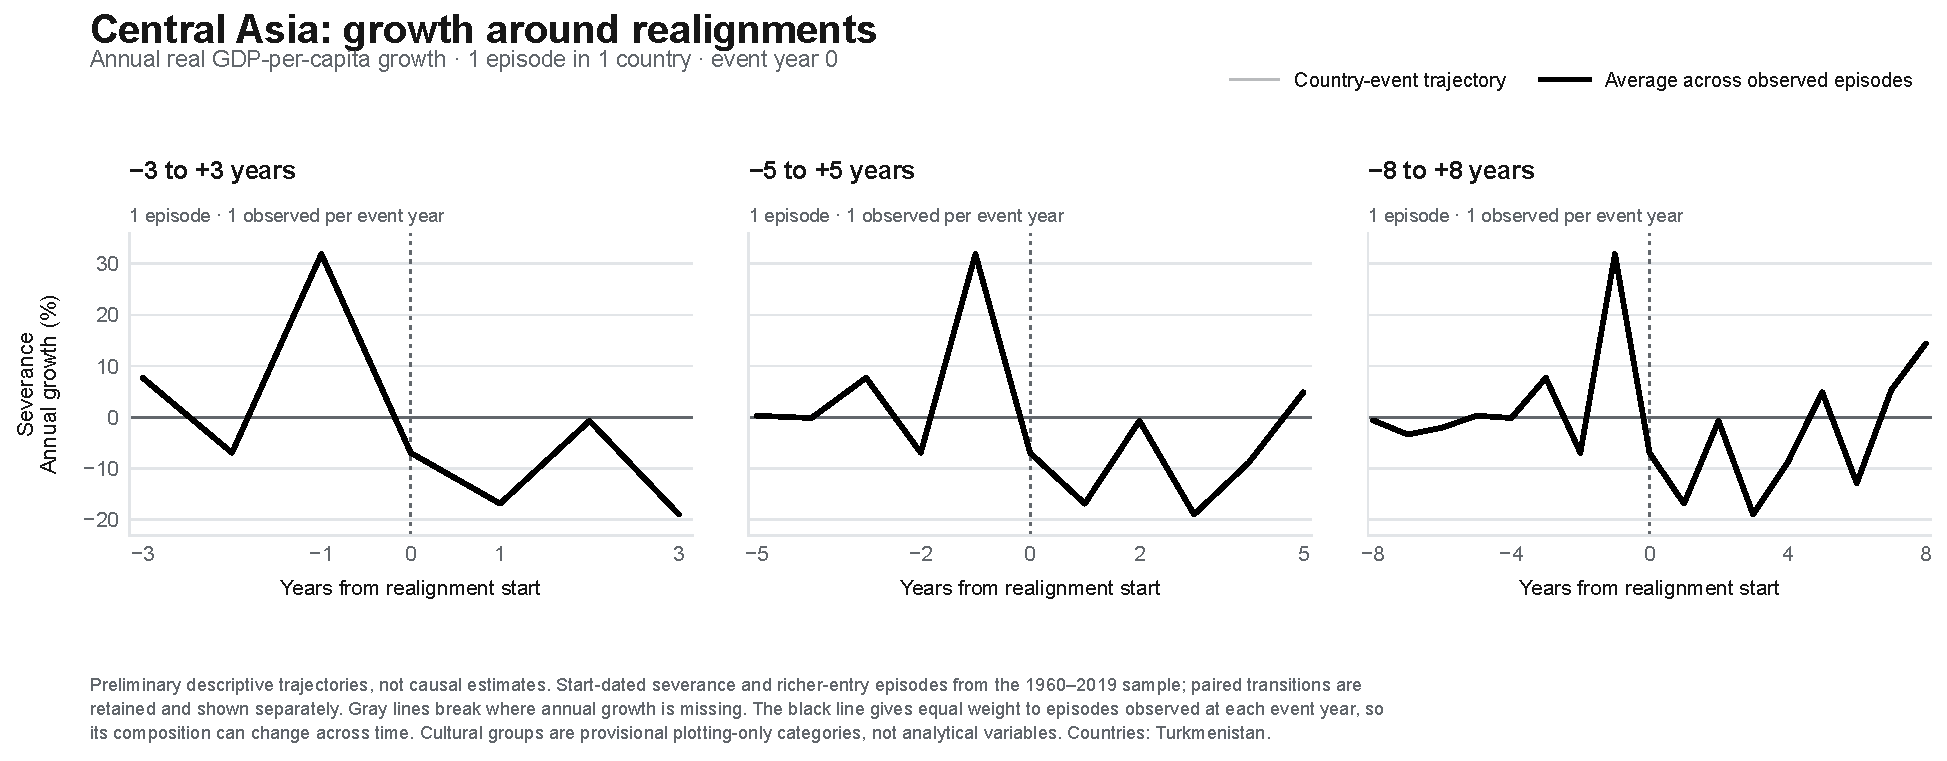
\includegraphics[width=\textwidth]{figures/event_time/central_asia_event_time_preliminary.pdf}
\caption{Event-time growth profiles: Central Asia. The single-episode average reproduces Turkmenistan's trajectory.}
\label{fig:event_time_central_asia}
\end{figure}

\begin{figure}[p]
\centering
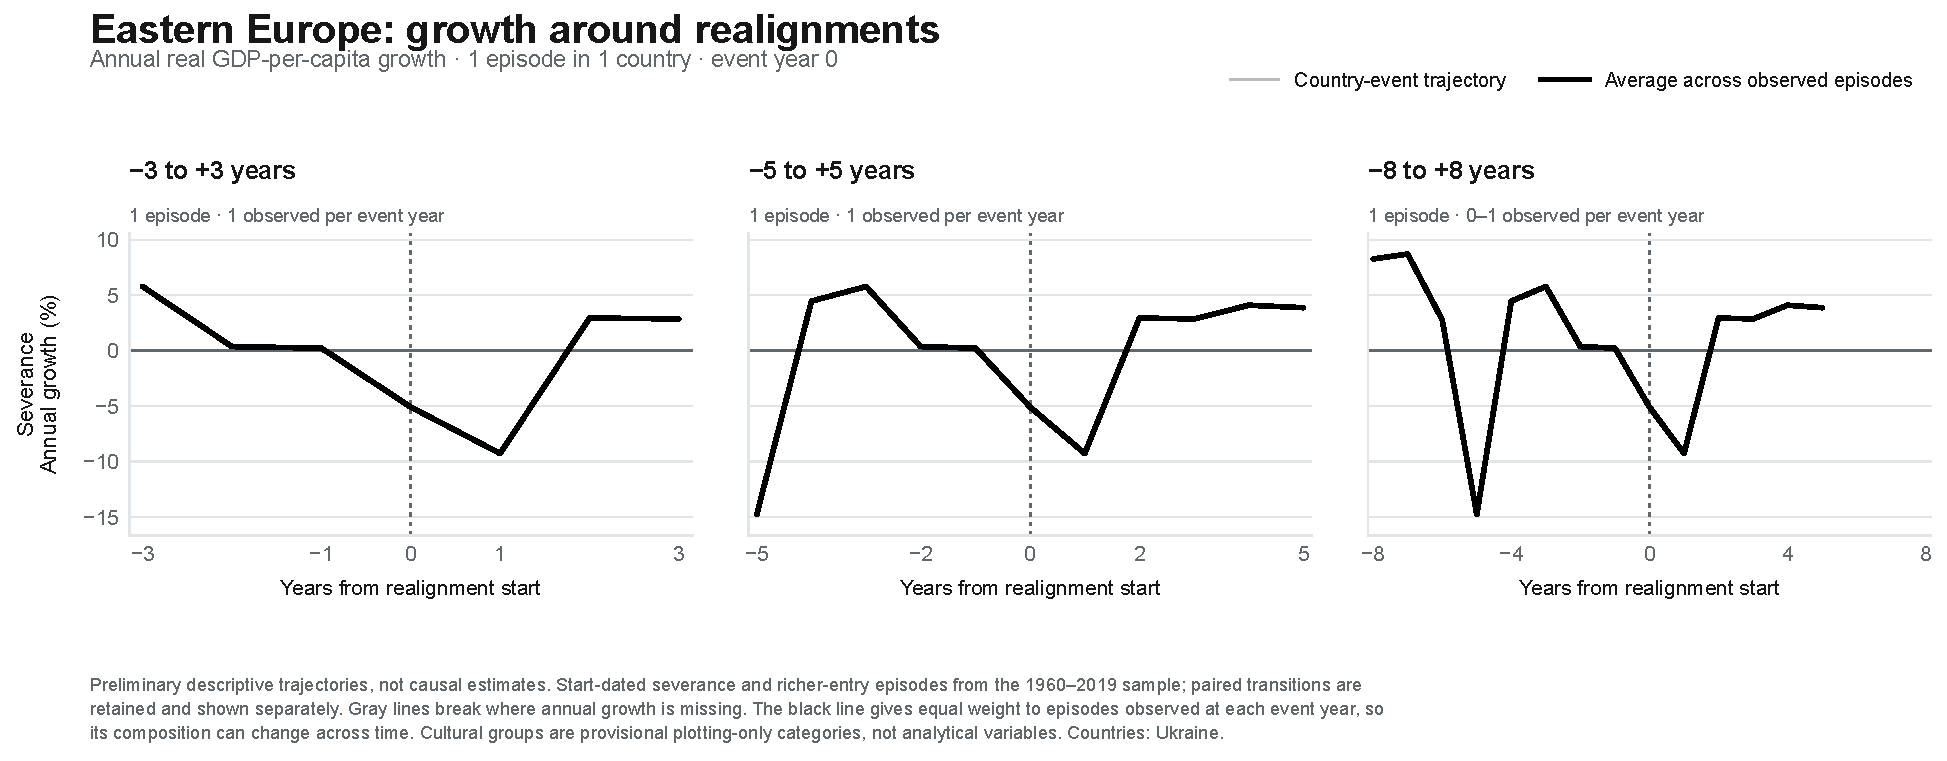
\includegraphics[width=\textwidth]{figures/event_time/eastern_europe_event_time_preliminary.pdf}
\caption{Event-time growth profiles: Eastern Europe. The single-episode average reproduces Ukraine's observed trajectory.}
\label{fig:event_time_eastern_europe}
\end{figure}

\clearpage

\subsection{Preliminary discussion}

For $H_1$, the turnover/formal-only and no-domestic-event rows without realignment have broadly similar mean growth and disruption frequencies, although both contain substantial disruption and acceleration. This pattern sits uneasily with a strong universal reading of the hypothesis. It cannot provide a causal falsification because the table implements neither matched-country comparisons nor the conditional null in equation~\eqref{eq:main}.

For $H_2$, the start-date severance and richer-entry aggregates have the predicted signs, and imposed severances retain the negative pattern. The severance growth sign changes across dates and after systemic-shift exclusion; the richer-entry acceleration-onset rate also varies by date. Wrong-sign outcomes and outcomes without realignment remain visible, leaving a mixed descriptive picture. Mean positive growth after entry does not by itself satisfy the registered acceleration definition. Similarly, an external shock alone does not produce a growth collapse in Rodrik's interactive account \parencite{rodrik_1999}.

For $H_3$, the cells cannot identify the proposed interaction. Deep domestic transformations coincide with both negative and positive outcomes, and the event cells containing both domestic change and realignment are very small. These frequencies establish neither necessity nor sufficiency, nor do they identify an interaction. The theory leaves power-structure transformation without realignment unrestricted; the 0.84 percent mean growth in that cell has no bearing on a signed prediction.

For now, the results serve chiefly to guide the next empirical steps. The timing audit and sensitivity checks point to interval dating, actual changes in material-capability flows, paired transitions, and alternative explanations involving war, commodity prices, financial crises, and policy change. Anomalous cases must remain in the data; recoding them to fit the framework would undermine the test. Step 7 regression estimates and Step 8 process tracing, matched comparisons, and independent double-coding remain necessary before a hypothesis verdict.

The results also inherit several limitations recorded in the research protocol. Open realignment judgments, including E020, E059, and E067, remain unresolved; 996 formal-candidate country-years retain unknown amendment content; post-2015 turnover remains unverified; and the sudden-stop component of disruption remains uncoded. Window-edge formation episodes cannot supply a prior growth regime, and independent reliability double-coding has yet to occur. Any conclusion is confined to the current preliminary coding state.

% =========================================================================
% 8. LIMITATIONS AND CONCLUSION
% =========================================================================
\section{Limitations and Conclusion}
\label{sec:discussion}

Four limitations of this research design should be acknowledged. First, \emph{major economic discontinuity} still requires operationalization: a disruption threshold along the lines suggested by \textcite{rodrik_1999} and a symmetric acceleration threshold along the lines of \textcite{hausmann_pritchett_rodrik_2005}. Second, the boundary between nominal regime change and genuine power-structure transformation is clear in principle \parencite{garciatrevijano2010,linz_stepan_1996}; coding it remains empirically demanding. Historical cases of state-apparatus restructuring \parencite{skocpol_1979} will guide the coding rules. Third, the framework is deliberately agnostic about normative evaluations of regimes. Its concern is the organization of power; normative desirability lies outside the classification. Fourth, entry into a richer sphere is partly endogenous because patrons often admit states that are already reforming. Causal identification must therefore rest on severances imposed by a patron's collapse or withdrawal.

The thesis attributes much of what is usually credited to ``regime change'' to external realignment: a change in the state's position within the international structure. Severance of a dominant-power relationship produces disruption, whereas anchoring the state in a richer sphere produces acceleration. Domestic political change that leaves the structure of political power untouched leaves the economy on its prior path. The empirical chapters will test these claims on matched pairs of countries.

\printbibliography

\end{document}
